\documentclass{ctuthesis/ctuthesis}
\usepackage{subfig}
\usepackage{amsfonts}
\usepackage{ieeetrantools}

\ctusetup{
	xdoctype = B,
	xfaculty = F8,
	mainlanguage = english,
	titlelanguage = english,
	title-english = {Autonomous Car Chasing},
	%title-czech = {Automaticke pronasledovani auta},
	department-english = {Department of Applied Mathematics},
	author = {Pavel Jahoda},
	supervisor = {Ing. Jan Čech, Ph.D.},
	supervisor-address = {Czech Technical University in Prague Faculty of Electrical Engineering  \\
	Center for Machine Perception},
	fieldofstudy-english = {Knowledge Engineering},
	keywords-czech = {samořídíci auto, RC auto, víceúlohové učení, autonomní řízení, hluboké učení, CARLA, simulace},
	keywords-english = {self-driving car, RC car, multi-task learning, autonomous driving, deep learning, CARLA, simulation},
	month = 5,
	year = 2020,
	specification-file = {images/zadani.pdf},
	front-specification = true
}

\ctuprocess

\begin{abstract-english}

A car chase is a scenario that requires dynamic maneuvers, fast reactions, and strategic trajectory planning. It tests the limits of an autonomous driving system.

We developed an autonomous driving system that can chase another vehicle using only images from a single RGB camera. At the core of the system is a novel dual-task convolutional neural network capable of simultaneously performing object detection as well as coarse semantic segmentation. The system has been firstly tested in CARLA simulation. We created a new challenging publicly available chasing dataset collected by manually driving the chased car. Using the dataset, we showed that the system benefits from using coarse semantic segmentation. The system that uses the semantic segmentation was able to chase the pursued car on average 10\% longer than other versions of the system. 

Finally, we integrated the system into a subscale vehicle platform built on a high-speed RC car and demonstrated its capabilities by autonomously chasing another RC car.


% We present a novel dual-task convolutional neural network capable of simultaneously performing object detection as well as coarse semantic segmentation. The network has been integrated into the system.

% We have developed an autonomous driving system that can chase another vehicle. Furthermore, we introduce a novel dual-task convolutional neural network capable of simultaneously performing object detection as well as coarse semantic segmentation. The network has been integrated into the system. 

% The system has been first tested in a CARLA simulation. Then, it has been integrated into a subscale vehicle platform attached to a high-speed RC car and has been evaluated by autonomously chasing another vehicle.


% A safe autonomous driving system must have fast reaction times to ultimately prevent accidents and crashes. A car chase is a situation that requires such fast reaction times.


% In our work, we introduce a fast novel dual-task convolutional neural network capable of simultaneously performing object detection as well as coarse semantic segmentation. Furthermore, we have developed an autonomous driving system that uses the dual-task neural network. The system has been integrated into a subscale vehicle platform attached to a high-speed RC car and has been evaluated by autonomously chasing another vehicle. The system architecture and results of the evaluation are presented. 

\end{abstract-english}



\begin{abstract-czech}
Pronásledování auta je situace, která vyžaduje dynamické manévry, rychlé reakce a strategické plánování trajektorie. Zároveň nám umožňuje testovat limity autonomního řízení.

Vytvořili jsme autonomní řídící systém, který dokáže pronásledovat další vozidlo pouze na základě RGB obrazu z jedné kamery. V jádru tohoto systému je nová víceúlohová konvoluční neuronová síť, která dokáže simultánně detekovat objekty a hrubě sémanticky segmentovat obraz. Tento systém byl nejprve otestován v simulátoru CARLA. Pro tyto účely jsme vytvořili nový veřejně dostupný pronásledovací dataset. Dataset byl vytvořen manuální jízdou pronásledovaného vozidla. Za použití tohoto datasetu jsme ukázali, že systém funguje lépe když využívá hrubou sémantickou segmentaci. Takový systém dokázal pronásledovat druhé vozidlo v průměru o 10\% déle než verze systému které sémantické segmentace nevyužívají.

Na závěr byl tento systém integrován do platformy nazvané \uv{subscale vehicle platform} připevněné na velmi rychlé RC auto na kterém byl systém testován pronásledováním dalšího RC vozidla.
\end{abstract-czech}

% Acknowledgements / Podekovani
\begin{thanks}
I would like to express my deep gratitude to my supervisor Assistant Professor Ing. Jan Čech, Ph.D. for his patient guidance and willingness to devote his time to this work. I would also like to thank ToMi team (Michal Bahník, Dominik Filyo, Martin Vlašimský, and others) who have assembled the subscale vehicle platform on a 1:5 RC car used as the chasing car. Furthermore, I would like to thank doc. Ing. Martin Hromčík, Ph.D. for lending me his 1:10 RC car that was used as the chased car.\par


Finally, I would like to extend my thanks to my parents for their support throughout my education and to my girlfriend Vanda for her support and for helping me film a promotional video of the autonomous car chase.
\end{thanks}

% Declaration / Prohlaseni
\begin{declaration}
		I hereby declare that the presented thesis is my own work and that I have cited all sources of information in accordance with the Guideline for adhering to ethical principles when elaborating an academic final thesis.
		
		I acknowledge that my thesis is subject to the rights and obligations stipulated by the Act No.\,121/2000~Coll., the Copyright Act, as amended. In accordance with Article~46~(6) of the Act, I hereby grant a nonexclusive authorization (license) to utilize this thesis, including any and all computer programs incorporated therein or attached thereto and all corresponding documentation (hereinafter collectively referred to as the ``Work''), to any and all persons that wish to utilize the Work. Such persons are entitled to use the Work in any way (including for-profit purposes) that does not detract from its value. This authorization is not limited in terms of time, location, and quantity.
\end{declaration}



\begin{document}
\bstctlcite{BSTcontrol}
\maketitle

\chapter{Introduction}
An autonomous car driving system capable of making fast and accurate decisions is important for making car transportation a safer activity. The reaction times of the system (especially in high speeds) have an impact on the human trust and acceptance of automated vehicles. The key aspects of driving autonomously include an understanding of the surrounding environment, detecting other cars, and interacting with them on the road. In this paper, we present a novel neural architecture that gives information about other cars as well as the surrounding drivable surface. We then test an autonomous driving system, that we developed, in these aspects by using a car chasing scenario. \par


A similar scenario -- car-following -- has been studied for more than half a century. Car-following models describe how vehicles should follow each other in a traffic stream. Frequently these theoretical models assume having precise data such as speed, distance, and acceleration at every timestamp \cite{car_following}. However, with the advancements of machine learning and computer vision more practical car-following models have been developed and tested. These models use sensors such as LIDAR and camera to estimate the distance between the two cars \cite{lidar_highway}. The estimated information is then used to maintain a safe distance between the two cars while following the trajectory of the front car. However, the car-following models have typically not been tested in scenarios involving high speeds and sudden fast acceleration and deceleration. \par
 
 
On the other hand, a car chase -- a vehicular hot pursuit of suspects by law enforcers -- typically involves high speeds and therefore dynamic driving maneuvers are necessary. In our scenario, a vehicle being pursued is driven by a person, while the vehicle that is chasing it is being controlled by an artificial intelligence-based system. Solving an autonomous car chasing problem requires a system that solves many sub-problems from computer vision, planning, and control theory. The system is an integration of the solutions to these sub-problems. The architecture of our system is similar to the DARPA Urban Challenge vehicles \cite{Bertha,darpa2,darpa_book} and consists of three parts: perception and localization, trajectory planning, and a trajectory controller. \par


The thesis has the following structure. First, a theoretical background of the chasing algorithm is outlined. This includes related work described in Section \ref{s:related_work} and also a description of each part of the system in Section \ref{s:method}. Then, an experiment Section \ref{s:experiments} follows. The section includes evaluation in CARLA -- an open-source simulator for autonomous driving research \cite{CARLA}. Additionally, it has real-world testing of the system deployed in a radio-controlled (RC) car. The real-world evaluation consists of two parts. First, it has an evaluation of the novel neural network's ability to detect objects and segment images. This is done using a collected dataset that will be presented in the experiment section. Second, it describes a live test chase in which the goal is to maintain a determined distance between two RC cars. However, unlike in the car following problem, following the same trajectory is not required. Finally, Section \ref{s:conclusion} concludes the thesis.




\chapter{Related Work}\label{s:related_work}
\section{Path Following}
A path is understood as a set of waypoints $w_0,\dots ,w_n$. Given a path, a moving vehicle with an initial position $p=w_0$ and an initial vehicle heading angle $\psi$. A path-following algorithm tries to change $\psi$ at each timestamp $i \in \langle 0,n\rangle$ to minimize the sum of cross-track errors. The cross-track error is a distance between the vehicle and the closest point on the path. Furthermore, it attempts to minimize the differences between the heading angles $\psi_i$ and the angle formed by waypoints $w_i$ and $w_{i+1}$ called the LOS angle $\phi$ \cite{path_following_evaluation}.\par

In 1985, Carnegie Mellon University \cite{pure_pursuit_orig} demonstrated the first autonomous path-following vehicle. It works by finding a look-ahead position on the path and subsequently calculating the vehicle's heading angle $\psi$ as a curvature $\kappa$ of an arc as depicted in Figure \ref{f:pure_pursuit}. Using the Pythagorean theorem and the fact that $\kappa=\frac{1}{r}$, it can be deduced that $\kappa = \frac{2\cdot x}{p^2}$. \par

\begin{figure}[]
    \centering
    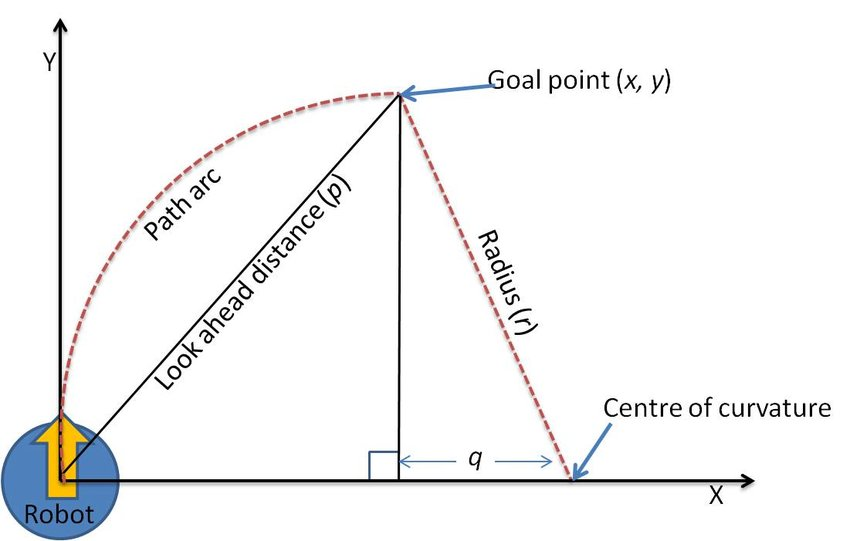
\includegraphics[width=0.8\textwidth]{images/Geometry-of-the-pure-pursuit-algorithm.jpg}
    
    \caption[The geometry of the pure pursuit path following algorithm]{The geometry of the pure pursuit path following algorithm, adopted from \protect\cite{nice_picture}}\label{f:pure_pursuit}
\end{figure}


A year later after introducing the pure pursuit algorithm, Carnegie Mellon University's Navlab was able to follow road at a maximal speed of 28 km/h \cite{navlab1}. Two decades later, autonomous cars were able to finish a 212 km off-road course at the DARPA Grand Challenge. The winning team introduced a novel path-following algorithm called Stanley method \cite{stanley_method}. Stanley method is a non-linear function that takes into account the difference between vehicle heading angle $\psi$ and the LOS angle $\phi$, gain parameter $k$, as well as the cross-track error $e$. Denoting the vehicle speed $u_i$ at time $i$, the steering control is given by:

\begin{equation}
steer = (\phi- \psi)_i + \arctan{\dfrac{k\cdot e_i}{u_i}}
\end{equation}


Solving the path-following problem is an important step to achieving a fully autonomous driving system. We acknowledge that there are many approaches and path following algorithms \cite{path_following_overview}, but for the sake of brevity, we have highlighted only two.
% they stated that the biggest challenge was computer vision

\section{Car Following and Chasing}
The goal of a car following problem is to maintain a predefined distance to a followed vehicle. Typically, the problem is solved with the goal of creating an autonomous convoy or a system capable of autonomously driving in highway traffic. Generally, in the car following problem it is expected that the leading car drives smoothly without aggressive turning or sudden braking. On the other hand, in the car chasing problem, the pursued car actively attempts to get away from the chasing car. While the chasing car also tries to maintain a certain distance between the two cars, the ultimate goal is not to lose the pursued car. For this reason, car chasing is a much more challenging problem. \par



The first scientists who attempted to solve the car chasing/following problem realised that an autonomous system with such capabilities needs to be able to perform many different tasks such as localization and planning. Many attempts focused on solving different parts of the system independently.\par

In the 1990s, the first attempts of localization of the ``lead'' chased car were made \cite{only_detection_and_tracking,also_only_car_tracking,night}. Schwarzinger et al.\ used a database of different car models to match the tracked vehicle to a vehicle model \cite{only_detection_and_tracking}. This gives information about the size of the pursued vehicle. Subsequently, this information is used to estimate the distance and relative position of the pursued car.


In 1991, Kehtarnavaz et al.\ developed the first autonomous car following system called BART \cite{BART_car_following}. The system was able to follow the leading car at 20 km/h speed. The system works by changing the velocity of the following car based on the velocity and the distance of the followed car. The authors stated that estimating the velocity of the lead car is a challenging problem. While a new Radar/Lidar sensor fusion solution for velocity estimation has been developed \cite{lidar_highway}, we address the issue by proposing a solution that controls the throttle based only on the distances between the two cars.


\subsection{Reinforcement Learning}
Reinforcement learning is a subfield of machine learning. It deals with what actions should an agent in an environment make to maximize some reward function. An example would be an agent driving a car on a road. In this scenario, the reward could be based on how long the agent is able to drive on the road. The idea is that eventually, the agent would learn from trial and error to match the correct responses (optimal steering value) based on the perceived state (where it is on the road).\par

With the rise of reinforcement learning in recent years \cite{alphago,deepstack,alphastar}, reinforcement learning based solutions for autonomous following and driving have been developed. Michels et al.\ developed an autonomous driving system capable of driving an RC car in an unstructured environment \cite{RL_autonomous_driving}. They used a supervised learning approach to estimate depth in an image. Then, they used a simulator to learn a control policy to steer based on the depth information from camera images. Zhu et al.\ developed a solution that imitates human-like velocity control during highway car following \cite{RL_humanlike,RL_velocity}.\par


Reinforcement learning algorithms are often trained (at least partly) in a simulator. This limits the ability of the system to drive based on the quality of the simulator. Pan et al.\ acknowledge the problem and address it by creating a network that converts non-realistic virtual image input into a realistic image with a similar scene structure \cite{synthetic_images}. Furthermore, they prove that a reinforcement learning agent benefits from training on more realistic images.\par


We have decided not to use a reinforcement learning approach. A major drawback of reinforcement learning is the black-box nature. On the other hand, since our system has three parts, we can analyze issues and figure out which part caused the issue, i.e., if it was caused by perception, planning, or control. This might not be possible using reinforcement learning. We also believe, that our approach is more suitable for possible hardware changes to the subscale vehicle platform attached to the RC car. 





\section{Target Following Using Unmanned Aerial Vehicles}
Unmanned aerial vehicles (UAV) are used in contemporary military operations. The use of UAVs has been steadily increasing for several years \cite{UAV_good_or_bad}. They have been used for remote mapping, data acquisition, target selection, and target chasing \cite{UAV_good_or_bad,UAV_use}. Target chasing and target following using UAVs is a similar problem to the car chasing problem. Generally, the architecture of an autonomous UAV is similar to the architectures used in autonomous vehicles \cite{target_following_alg,uva_tracking_formula}. It is usually divided into three parts: perception and localization, planning, and a controller. \par

There are two main differences between chasing a target with a UAV compared to vehicle chase. Firstly, UAV moves in more directions, which also means that altitude control is necessary. Secondly, frequently there is an assumption that no obstacles would prevent the UAV to move in all directions \cite{target_following_alg,uva_tracking_formula,rotorcraft}. \par


As an example of an autonomous UAV target chasing, Telière et al.\ developed an autonomous quad-rotor UAV that chases a moving RC car \cite{uva_tracking_formula}. They set the camera attached to the UAV in a way that the heading vector of the camera is perpendicular to the ground. Then, they estimate the distance error between the center of the image and the moving target. Finally, with the assumption that there are no obstacles, the system moves the UAV to minimize the measured error. This is similar to our approach as we also move the chasing car based on estimated distance between the chasing and chased car. On top of that, our system performs semantic segmentation and plans a trajectory based on information about the surrounding environment. 



\chapter{Method}\label{s:method}
\section{Overview}
\begin{figure}[]
    \centering
    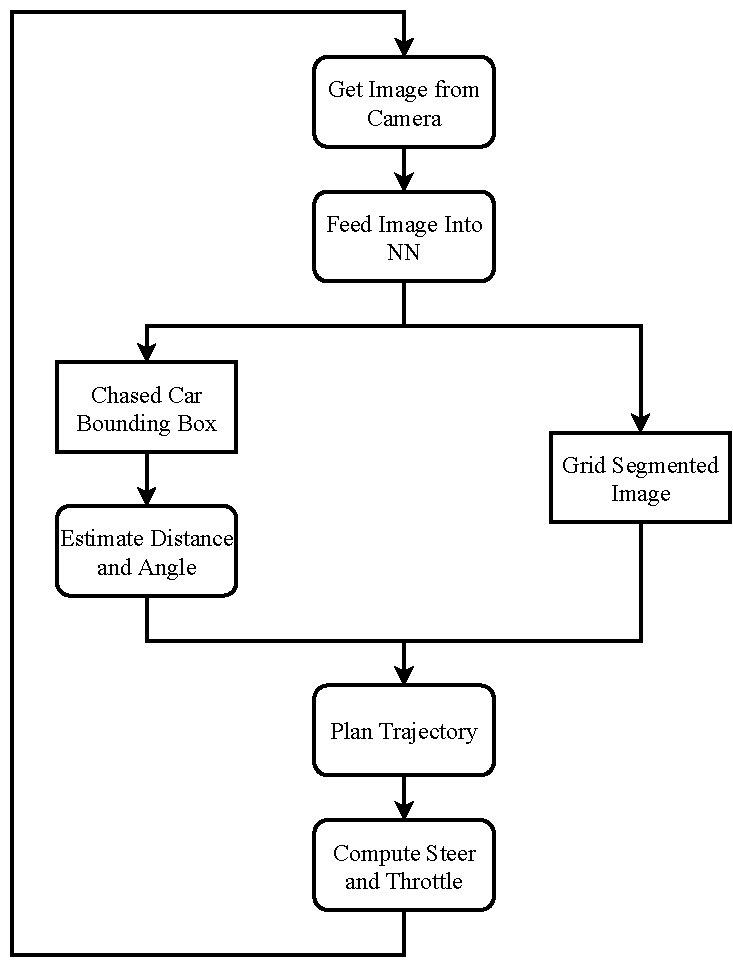
\includegraphics[width=0.7\textwidth]{images/bachelor_diagram.pdf}
    \caption{Simplified overview of the autonomous driving system}\label{f:overview}
\end{figure}

The system architecture is divided into three parts: perception and localization, trajectory planning, and a trajectory controller. The architecture is depicted in Figure \ref{f:overview}. \par


In the perception part, we introduce a novel neural network that detects objects and segments an image at the same time. It is able to find a 2D bounding box of the chased car. Furthermore, it segments an image into a coarse grid of $S\times S$ cells and makes a classification about each cell whether it is a drivable surface or not. The detection and segmentation are done with a single pass of the image through the neural network. \par


Then, we estimate the angle and distance between the two cars based on the detected bounding box of the chased car. In case no bounding box is found we extrapolate the distance and angle. \par


After the perception and localization, the trajectory is planned. At this stage, we take advantage of the image segmentation. If only a drivable surface is between the two cars, we try to drive straight at the last position of the chased car. Otherwise, we use the image segmentation and find a direction where it is possible to drive and that is also closest to the position of the chased car. \par


Finally, with the trajectory planned, we calculate the steer and throttle to drive the vehicle. We use a PID controller \cite{PID_orig} to control the throttle. It takes into account the current as well as the previous distances between the chasing and chased car. A Pure Pursuit \cite{pure_pursuit_orig} inspired algorithm is developed to control the steering. \par

Details of the method will be described in the following sections.




\section{Computer Vision}
\subsection{Dual-task Neural Network}
In this section, we introduce a novel neural network that solves two problems at once -- object detection and semantic segmentation. \par


The neural network shares the same backbone for both tasks -- a 53 layer feature extractor called Darknet-53 \cite{YOLOv3}. Attached to the feature extractor are two sets of layers -- one that gives the output for the object detection and the other that gives an output for the image segmentation. The architecture of the neural network is depicted in Figure \ref{f:dual_task}.\par


\begin{figure}[]
    \centering
    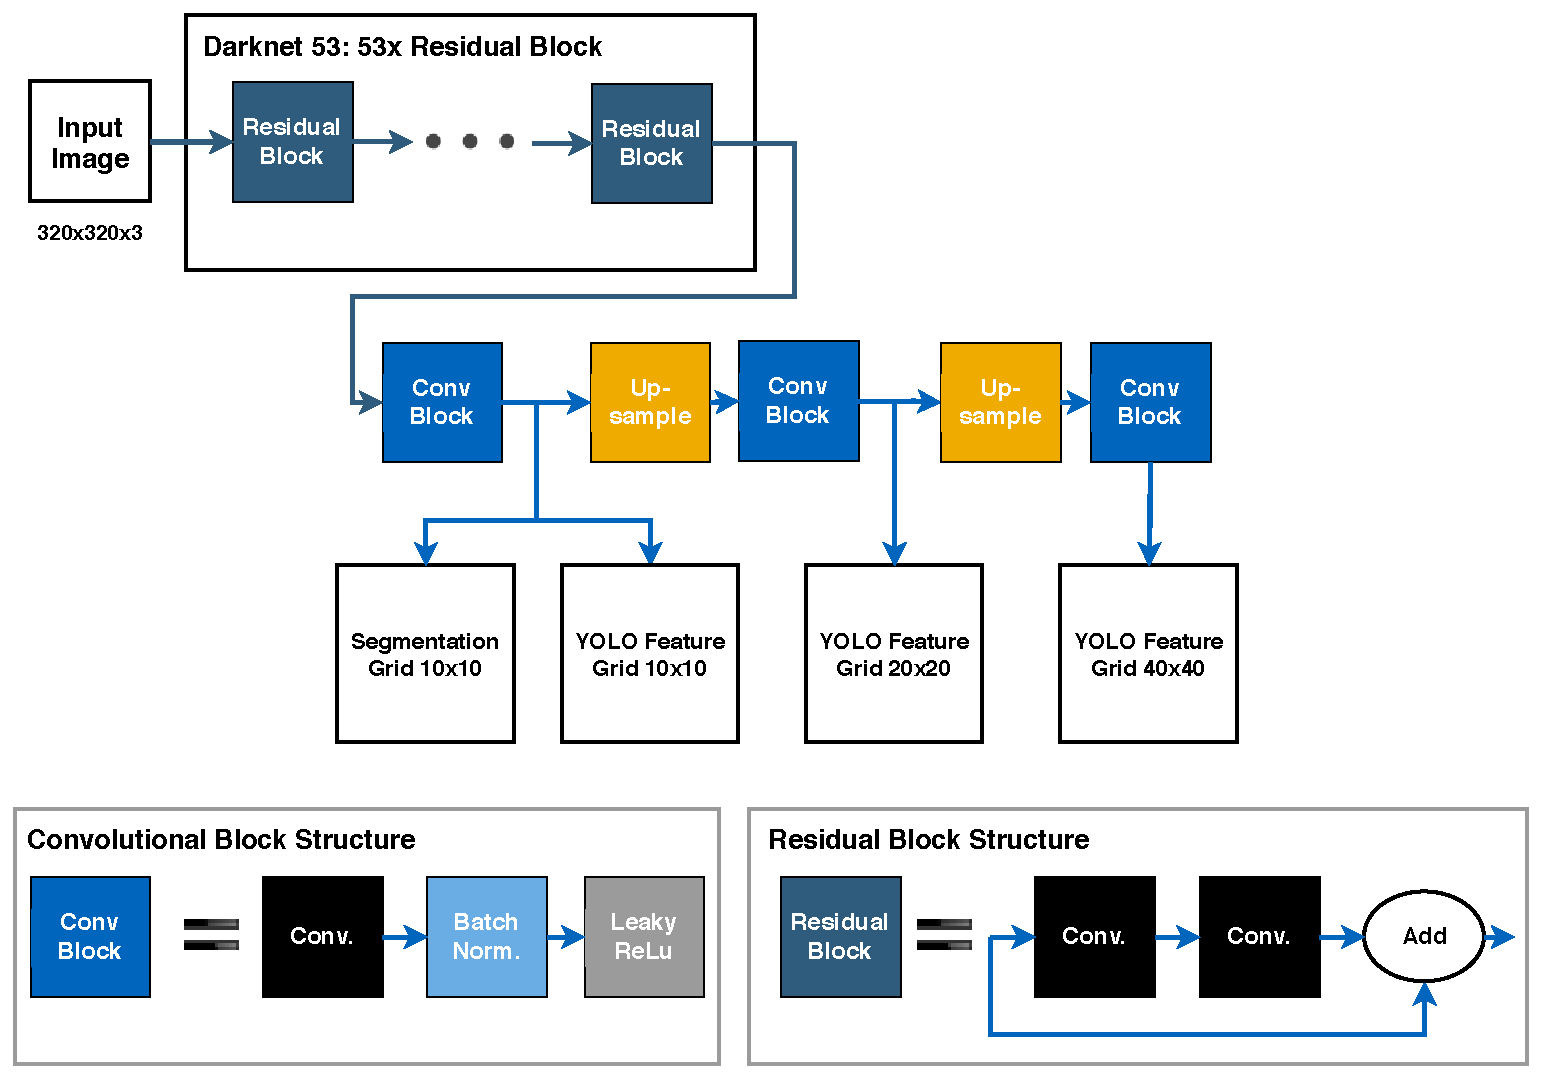
\includegraphics[width=1\textwidth]{images/network_architecture.pdf}
    
    \caption[Architecture of the novel dual-task convolutional neural network]{Architecture of the novel dual-task convolutional neural network. The three YOLO Feature Grids are used to predict bounding boxes at 3 different scales (described in Section \ref{s:detection}). The Segmentation Grid is the output of the coarse semantic segmentation. }\label{f:dual_task}
\end{figure}



The network is trained by alternating optimization -- in every second batch, the network is optimized only for detection, while the segmentation is optimized in the remaining batches. The neural network uses different loss functions depending on the batch. During training, when the network receives a training batch of data for semantic segmentation, the output for the object detection is ignored, and consequently, only the shared layers (the feature extractor) and the segmentation layers are trained. Equivalently, when the network gets a batch containing object detection data, it updates the weights only on the shared layers and the detection layers. \par


During inference, the network works as follows. It is given an image, which passes through the network just once. From this, we get an object detection output as well as the semantic segmentation output. This means that while the training is slightly slower than training a single-task neural network, the extra cost is negligible during inference since the backbone features are shared. \par


For autonomous driving, the neural network architecture has many advantages over using two separate networks. First, as was mentioned, it is much faster. That is crucial when driving autonomously because we want to process as many frames per second as possible and have fast reaction times to ultimately prevent accidents and crashes. Second, it uses less memory, because most of the network weights are shared. This is potentially beneficial for the overall speed since more RAM is available, less disk swapping is required. Finally, it makes integration of the detection and segmentation into our autonomous RC car system, having limited computational power, a lot simpler.




\subsection{Bounding Box Detector} \label{s:detection}
In our work, a bounding box is the smallest 2D axis-aligned rectangle that encloses all pixels belonging to the chased RC car in an image. The detection is performed by a convolutional neural network \cite{CNN_Lecun} with YOLOv3 neural network architecture \cite{YOLOv3}. \par 
The first version of the YOLO published in 2015 \cite{YOLO}, made a great improvement to the previous state-of-the-art object detection solutions with its ability to predict bounding boxes of multiple object classes with incredible inference speed. It works by reasoning globally about the whole images and all its object classes. \par


\begin{figure}[h!]
    \centering
    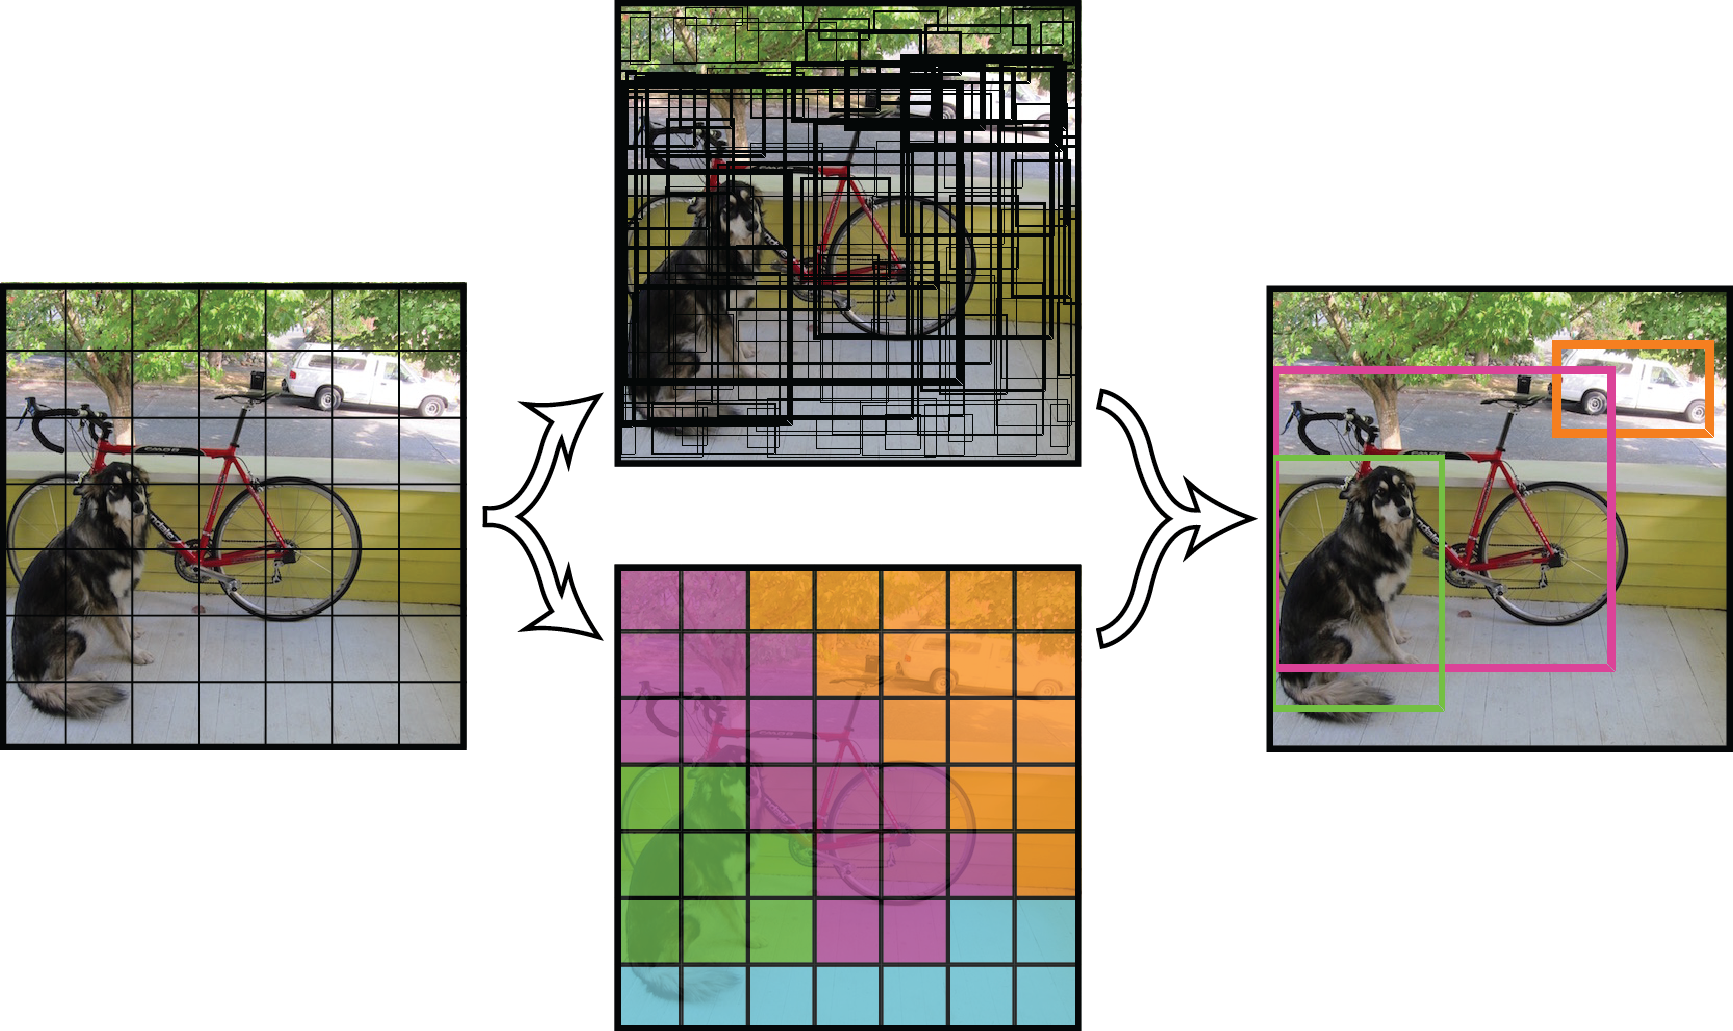
\includegraphics[width=0.8\textwidth]{images/YOLO.png}
    
    \caption[Diagram showing YOLO neural network mechanism]{Diagram showing YOLO neural network mechanism, adopted from \protect\cite{YOLO}}\label{f:YOLO}
\end{figure}

The YOLO neural network divides an image into $S\times S$ grid of cells. Each cell makes $K$ bounding box predictions. Each prediction is a vector containing width, height and the $(x,y)$ coordinates of the center of the bounding box. For each object in the image, the cell that has the center of the object inside is responsible for predicting its bounding box. This can be seen in the top middle image in the Figure \ref{f:YOLO}. Concurrently, each cell outputs $C$ values where each value represents a predicted probability of whether an object from a class $C_i$ is in the cell. The resulting class map from these predicted probabilities is seen in the bottom middle image in the Figure \ref{f:YOLO}. Both of these predictions -- the class probabilities and the bounding box predictions -- are then used together to make detection and classification of the objects in the image.
\par

During training, YOLO optimizes a multi-task loss function. It concurrently optimizes the bounding box regression as well as the class probabilities predictions.


Two years after introducing YOLO, the second version of called YOLO9000 \cite{YOLO9000} was introduced. In the first version of YOLO, each cell makes $K$ bounding box predictions of a random size. This was improved by calculating the expected bounding box sizes by clustering the bounding boxes of the training set. These expected bounding boxes are called anchors or priors. Furthermore, YOLO9000 also uses different network architecture called Darknet-19 and enables detection on different image sizes. \par


The third version of the YOLO architecture \cite{YOLOv3} improves YOLO in two main ways. Firstly, it adds more layers to the Darknet network architecture. Secondly, inspired by Feature Pyramid Networks \cite{FPN}, it predicts boxes at 3 different scales. To be specific, instead of dividing the image into $S\times S$ grid of cells, YOLOv3 divides it into $S\times S$, $(S\cdot2)\times (S\cdot2)$ and a $(S\cdot4)\times (S\cdot4)$ grid of cells. This helps the neural network to detect objects across a larger range of scales.


In our work, we have used the YOLOv3 detector pre-trained on a COCO dataset consisting of more than 330 000 images with objects from 80 different classes \cite{COCO_dataset}. The neural network was fine-tuned on our dataset that has 460 images of the chased RC car. The dataset is described in Section \ref{s:detection_dataset}. During fine-tuning, only the final layers that follow the Darknet-53 feature extractor were updated.




\subsection{Angle and Distance Estimation}
One of the most crucial information when chasing another vehicle is its relative angle and distance to the chasing car as sketched in Figure \ref{f:chasing_diagram}. In our work, we are estimating the angle between the heading vector of the chasing car and the vector pointing from the center-front of the chasing car to the center of the back of the pursued car. Furthermore, we estimate the distance between the two cars. To be specific, the distance $d$ between the front of the chasing car and the center of the back of the pursued car. \par


\begin{figure}[]
    \centering
    \includegraphics[width=0.7\textwidth]{images/ChasingDiagram.png}
    
    \caption[Angle and distance estimation 2D overview]{Angle and distance estimation: Blue chasing car on the left and pursued car on the right. It shows the ground truth distance $d$ and the angle $\varphi$ we are estimating using a camera mounted on the chasing car }\label{f:chasing_diagram}
\end{figure}

Figure \ref{f:chasing_diagram} shows this problem in a simplified 2D view. To estimate the distance and the angle of the car from an image, we took advantage of existing solutions solving PnP (Perspective-n-Point) problem. The PnP is a problem of estimating position and orientation of a camera from a set of $n$ known 3D points, their corresponding 2D projections in the image, and the calibrated intrinsic camera parameters. This leads us to the following camera projection equation: \par


\begin{equation}
s\,\mathbf{p_{image}} = \mathbf{K}\,[\,\mathbf{R}\, |\, \mathbf{T}\, ]\, \mathbf{p_{model}}
\end{equation}

Where $s$ is a scaling parameter since $\mathbf{p_{image}}$ and $\mathbf{p_{model}}$ are in homogeneous coordinates. The $\mathbf{p_{image}}$ are the coordinates of the points in the image, $\mathbf{p_{model}}$ are the 3D model coordinates, $\mathbf{K}$ is the matrix of intrinsic camera parameters and $\mathbf{R}$ and $\mathbf{T}$ are the rotation and translation we are estimating. This can be further rewritten as: \par


\begin{equation}
s\begin{bmatrix}u\\v\\1\end{bmatrix} = \begin{bmatrix}
f_x & \gamma & u_0\\
0 & f_y & v_0\\
0 & 0 & 1
\end{bmatrix}\begin{bmatrix}
r_{11} & r_{12} & r_{13} & t_{1}\\
r_{21} & r_{22} & r_{23} & t_{2}\\
r_{31} & r_{32} & r_{33} & t_{3}\\
\end{bmatrix}
\begin{bmatrix}x\\y\\z\\1\end{bmatrix}
\end{equation}

In our case, the image points $p_{image}$ are the bounding box corners of the detected car. We also estimated the model coordinates $p_{model}$ by measuring the width and height of the chased RC car. We assume that the bounding box encloses only the corresponding image points, i.e., the back of the RC car. We acknowledge that the assumption does not always hold true, but we found the resulting inaccuracies to be negligible. Finally, the intrinsic camera parameters such as focal lengths $f_x$ and $f_y$ were taken from the manufacturer calibration of the ZED camera. Then, we plugged these values into an OpenCV \cite{opencv_library} library function SolvePnP (with CV\_ITERATIVE flag) which gave us the translation and rotation vectors. Afterwards, we calculated the distance $d$ by calculating the Euclidean distance between the translation vector $\mathbf{T}$ and the origin. Similarly, we extracted the desired estimated angle $\varphi$ by calculating arc tangent between the negative values of $x$ and $z$ components of the translation vector $\mathbf{T}$. \par

Finally, since we are using a stereo camera and the camera lens which was used is not in the center of the front of the car, we converted the calculated angle and distance as if the camera was in the center of the front of the car. We achieve this with a simple triangulation. Note that only monocular is made. More precise estimation using stereo vision could be achieved, however, for higher computational cost.




\subsection{Angle and Distance Extrapolation}
In the previous section, we have described how we estimate angle distance based on the bounding box of the chased car. However, in some cases the detector is unable to detect the object in the image due to poor lighting conditions in the scene, or because the pursued vehicle is only partially visible/non-visible due to some object occluding it. Furthermore, there are cases when the chased car is out of the field of view. In these cases, we need to make a reasonable prediction about the position of the chased car. \par


We extrapolate the angle and the distance of the chased car based on the previous estimates. At the heart of the extrapolation algorithm is an exponential moving average. In fact, we use just six variables to store information about the whole history of estimated angles and distances. The idea will be explained by the process of extrapolating distances. The angle extrapolation is done similarly. \par


For every frame, we update the exponential moving average variable using the following equation:\par


\begin{equation}
    \hat{e_{i}}=
    \begin{cases}
      \alpha\cdot d_i + (1-\alpha)\cdot \hat{e}_{i-1}, & \text{if bounding box found} \\
      \alpha\cdot d_{extrapolated} + (1-\alpha)\cdot \hat{e}_{i-1}, & \text{otherwise}
    \end{cases}
\end{equation}

Where $\hat{e_{i}}$ is the exponential moving average variable at $i$th frame, $\alpha$ is a value in range [0,1] that sets the weight of the last predicted distance. In our algorithm, we have chosen value $\alpha=0.5$. \par

If the chased car is detected at $i$th frame, we set $d_i$ equal to the predicted estimate received from the PnP solver. We then update the variable $\hat{e_{i}}$ using the estimate $d_i$ and subsequently output the variable $d_i$ as our estimate for $i$th frame. In case no bounding box was detected, we update the $\hat{e_{i}}$ variable with $d_{extrapolated}$ variable that is computed using the following linear extrapolation equation:


\begin{equation}
d_{extrapolated} = 2\cdot d_{i-1} - d_{i-2}
\end{equation}

Afterwards, we output the variable $\hat{e_{i}}$ as our estimate for $i$th frame in case no bounding box was detected. Then, we set $d_i = d_{extrapolated}$ for future linear extrapolation computations. Finally, each extrapolated angle is processed by a saturation block that limits the output values. The saturation limits are -175 and 175 degrees. \par


This method allows us to extrapolate the angle and the distance very fast in a $\mathcal{O}(1)$ time and space complexity with almost no overhead.




\subsection{Image Segmentation}\label{s:Image_Segmentation}
In comparison to the semantic segmentation that links each pixel of the image to a class label, we segment the image into a coarse grid of $S\times S$ cells. Each cell linked with a class label. In our work, we have chosen $S=10$ and only two classes. The first class represents a drivable surface while the second class is everything else. \par


\begin{figure}[h!]
    \centering
    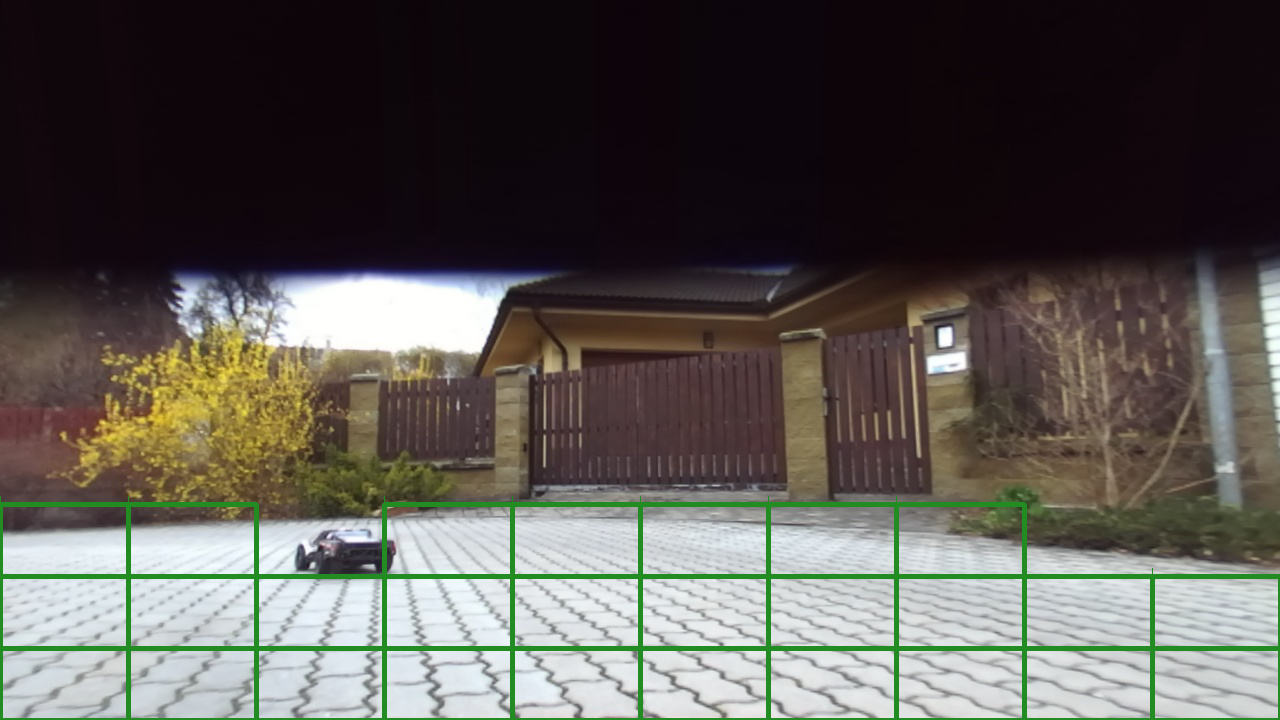
\includegraphics[width=0.8\textwidth]{images/segmented_image.png}
    
    \caption[Segmented image from the RC car's camera]{Segmented image from the RC car's camera. The image is segmented into $10\times 10$ grid of cells where the green cells represent a drivable surface. The image is taken from our test set}\label{f:segmented_image}
\end{figure}

To create a labeled dataset, we used semantic segmented images (an image that has each pixel of the image linked to a class label). Then, we calculate the number of pixels in a cell that belong to the class representing the drivable surface. If the percentage of these pixels is higher than $P$ percentage of all the pixels in the cell, we assign the cell said label. In our work, we have chosen $P=50\%$.\par


Since we have only two classes we can represent each cell label as binary 1 or 0. For this reason, we have chosen the logistic loss function to train the network. \par

\begin{equation}
L_{log} = -\dfrac{1}{N} \sum_{i=1}^{N} y_i \cdot \log_{} (\hat{y_i}) + (1 - y_i) \cdot \log_{} (1-\hat{y_i})
\end{equation}

Where $N$ is the number of images per batch, $\hat{y_i}$ are the predicted segmentation values of the neural network for the $i$th image in the batch and $y_i$ are its labels. 




\section{Control And Planning}
In this section, we will explain how we control the steering and throttle of the vehicle based on the extracted information from the camera. Conversely to many algorithms \cite{Broggi2013,Werling2010}, we control steering and throttle separately. Steering control is inspired by pure pursuit algorithm and throttle is controlled by a PID controller.


\subsection{Pure Pursuit Inspired Algorithm} \label{sec:pure_pursuit}
Pure pursuit algorithm is a path tracking algorithm that moves a vehicle from its current position to some look-ahead position on the path. The algorithm was invented in the 1980s as it was used in the first demonstration of an autonomous vehicle capable of following a road using imagery from a black and white camera \cite{pure_pursuit_orig}. The goal of the demonstration was to keep the vehicle centered on the road while it was driving at a constant speed.\par


The algorithm works as follows. Firstly, it finds the goal point on the path. Then, it transforms the goal point to vehicle coordinates, and finally, it calculates the curvature that will drive the vehicle to the look-ahead position on the path. \par


In our work, we were inspired by the algorithm. As opposed to the pure pursuit algorithm settings, our car does not move at a constant speed. Secondly, we are not following a path, but rather chasing a moving RC car. Therefore, every time we process an image from the camera, we update our goal position. But unlike in the path-following algorithm, the target position is updated with respect to the current position of the chased RC car rather than to a position on a path. \par
Conversely to the pure pursuit algorithm, we do not calculate the curvature to control the steering. That is because we need to update the steering every frame based on the position of the chased RC car and take more aggressive turns to chase the pursued vehicle. In our algorithm we calculate the steering value with the following function:

\begin{equation}steer = (\cfrac{\varphi}{\textrm{180}})^{2}\end{equation}

Value $\varphi$ represents the angle between the chasing and the chased car shown in the Figure \ref{f:chasing_diagram}. The $steer$ variable is in [-1, 1] range, where -1 and 1 represent the highest left-turn and right-turn steering angle the car can make respectively. We square the result of the division because the steering control on the RC car is non-linear. We do not square the division in the CARLA simulation.




\subsection{Semantic Segmentation Based Planning}
During inference, we use the coarse segmented grid as depicted in Figure \ref{fig:segmentation_planning}. First, we construct a line segment from the center of the bottom side of the image to the bounding box of the detected car. If this line segment goes only through cells that are drivable, the trajectory planning phase stays unchanged and we try to follow the car directly as described in Section \ref{sec:pure_pursuit}. If that's not the case, we repeat the line segment construction. This time, however, the line segment goes from the center of the bottom side of the image to other cells on the same horizontal line as the bounding box of the car. When we find a line segment that goes only through cells with drivable surfaces and that is closest to the RC car, we try to drive the car in this direction until it is possible again to chase the car directly.

\begin{figure}[]
    \centering
    \subfloat[First proposed path]{{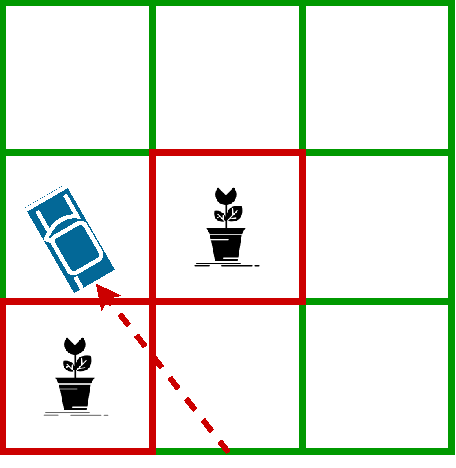
\includegraphics[width=0.3\textwidth]{images/dia1.pdf} }}%
    \quad
    \subfloat[Second proposed path]{{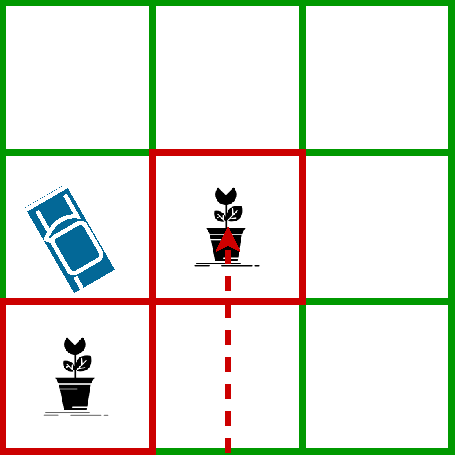
\includegraphics[width=0.3\textwidth]{images/dia2.pdf} }}%
    \quad
    \subfloat[Third proposed path]{{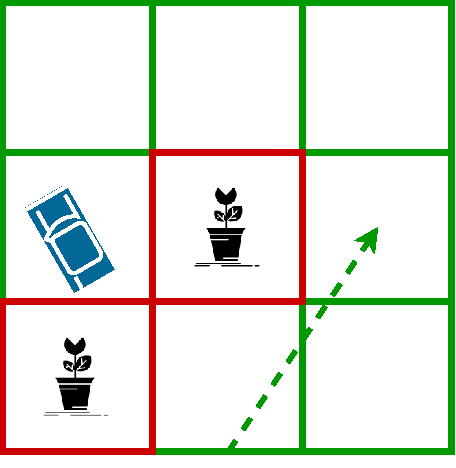
\includegraphics[width=0.3\textwidth]{images/dia3.pdf} }}%
    \caption[Example of a coarse semantic segmentation based planning using $3\times 3$ grid of cells]{Example of a coarse semantic segmentation based planning using $3\times 3$ grid of cells. First, the algorithm checks if it is possible to drive directly after the car \textbf{(a)}. This is not possible as the constructed line segment goes through a non-drivable grid cell. Then, the remaining cells on the same row as the detected car are checked \textbf{(b,c)}. The algorithm finally proposes a direction represented by a line segment that goes only through drivable surfaces and that is closest to the direction of the chased car \textbf{(c)}.}%
    \label{fig:segmentation_planning}%
\end{figure}

\subsection{PID Controller}
Despite being introduced in the 1940s, the PID controller is the most common control algorithm. In a 2002 survey of over 11 000 controllers from various industries, it was found that 97\% of regulatory controllers utilize PID feedback \cite{PID-usage}. 

In our work, we use a PID controller to control the throttle of the chasing autonomous car. As the name suggests it can be described with the following equation:

\begin{equation}
throttle = P+I+D    
\end{equation}
Term $P$ called the proportional term is equal to a value proportional to the current error value $\varepsilon_i$. In our case, the error value is $\varepsilon_i = d_i - d_{desired}$, where $d_i$ is the estimated distance between the chasing and the chased car, and $d_{desired}$ is the desired distance between the two cars that we are trying to maintain. Equivalently to the terms $I$ and $D$, the term $P$ is equal to a value multiplied by a weight $w_p$ which indicates the influence and importance of the term. Therefore, the term $P$ is described as $P = \varepsilon_i\cdot w_p$ \par


Term $I$ refers to the integration term. It integrates the errors over time. In our case, if the distance between the two cars continues to stay too large for a prolonged period, this term increases its value. It is equal to $I = w_i\cdot \sum_{j=(i-K)}^{i} \varepsilon_j$, where K is the number of frames representing the time we want to consider from the current frame. We used $K = 300$, which corresponds to the last 10 seconds.\par


The last component of the equation -- $D$ refers to the derivation term. Its purpose is to decrease the rate of change and decrease oscillations of the error value. In our work $D = w_d\cdot (\varepsilon_i-\varepsilon_{i-1})$. \par


To make the PID controller usable based on the dynamics of the system, the weights of the three components must be set. We have picked different weights for the CARLA simulation and the RC car. In the CARLA simulation, we have analyzed over a hundred sets of weights and picked the one that resulted in the lowest average error ($\varepsilon = d - d_{desired}$). These values were $w_p=0.1$, $w_i=0$ and $w_d=1$. For the RC car, we have chosen the values based on trial and error. They were $w_p=0.25$, $w_i=0$ and $w_d=0.07$. Finally, we saturate the output to the [0, 1] range. \par


The reason for choosing $w_i=0$ is pretty simple. While higher value of $w_i$ had a positive effect on the average error, it caused the car to crash into the chased car. In many cases, if the car was not catching up it made the car drive very fast and when it reached the desired distance, the car didn't slow fast enough resulting in a crash. Lowering the number of frames the integration part considers, did slightly help this issue. However, we decided not to take the risk of breaking a very expensive subscale vehicle platform attached to the RC car.



\chapter{Experiments}\label{s:experiments}
\section{Simulation}
\subsection{CARLA Environment}
All the simulation experiments were performed in CARLA -- an open-source simulator for autonomous driving research \cite{CARLA}. The experiments were done in CARLA version 0.9.8. CARLA has a wide selection of sensors including camera, segmentation camera, LIDAR on so on. It provides multiple maps with an urban layout. Users can control the weather, as well as many different actors (vehicles, pedestrians) at the same time. \par




\subsection{Experiment Setup}
In our work, we chose Tesla Model 3 as the chased car and Jeep Wrangler Rubicon as the chasing car. In each experiment, the pursued Tesla Model 3 was placed in front of the autonomously driven Jeep, as shown in Figure \ref{fig:CARLA}. At each frame, we simulated a bounding box detection of the chased car. We did this by projecting the ground truth world coordinates of the chased vehicle bounding box to the camera image coordinates. Then, we randomly perturbed the bounding box by adding random exponential noise proportional to the size of the bounding box. Furthermore, we simulated detection failure (false negative) in 10\% of the frames. The detection was also not provided when the chased car was out of the field of view.\par

All the experiments were performed in a synchronous mode in which the simulation waits for the sensor data to be ready before sending the measurements as well as halts each frame until a control message is received \cite{CARLA}. \par

\begin{figure}[]
    \centering
    \subfloat[View from the stereo camera attached to the chasing car]{{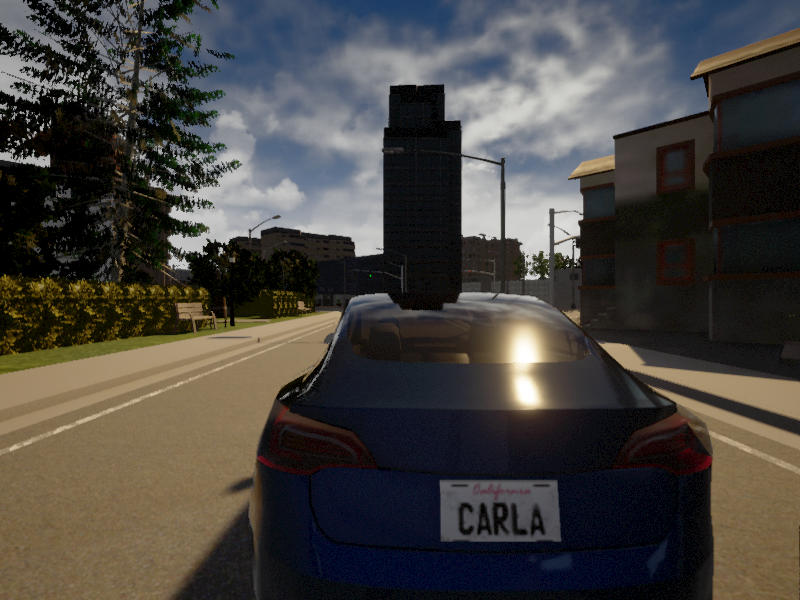
\includegraphics[height=4.3cm]{images/CARLA_camera_view.png} }}%
    \qquad
    \subfloat[View from above]{{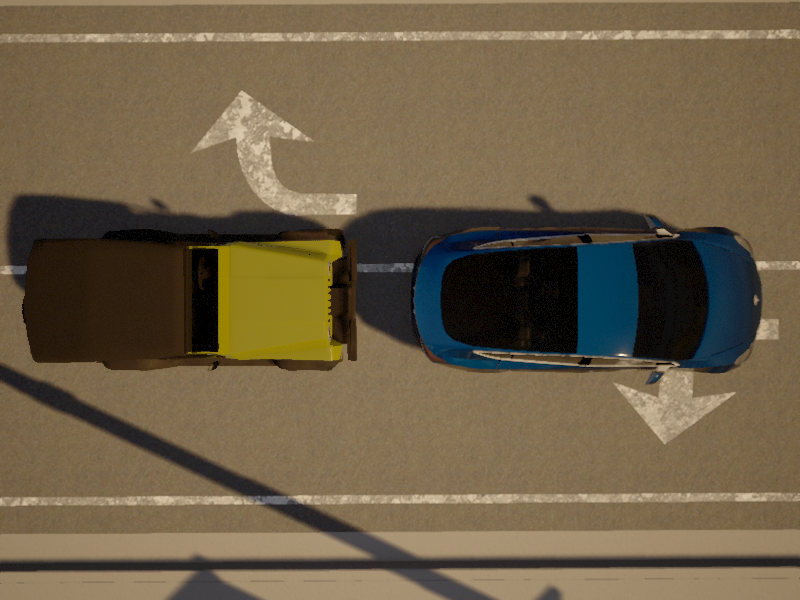
\includegraphics[height=4.3cm]{images/CARLA_top_view.png} }}%
    \caption{Two images showing the beginning of a CARLA experiment from two different perspectives}%
    \label{fig:CARLA}%
\end{figure}



%\footnote{Available at \href{https://github.com/JahodaPaul/autonomous-car-chase}{https://github.com/JahodaPaul/autonomous-car-chase}}

\subsubsection{Driving Dataset} \label{s:drivingDataset}
To perform the experiments we first collected a driving dataset \cite{my_github}. We used the Tesla Model 3 and manually drove it around the city using connected steering wheel and pedals Hama uRage GripZ \footnote{\href{https://www.hama.com/00113754/urage-urage-gripz-racing-wheel}{https://www.hama.com/00113754/urage-urage-gripz-racing-wheel}}. As the car was driven, its location and orientation were recorded at every frame. This way, we have collected a database of 20 different drives with varying difficulty (in a sense of chasing the car). We used this database to evaluate the autonomous driving system. At the beginning of the following experiments, a chasing car was placed half of a meter behind the chased car. Then, we updated every frame the location and orientation of the chased car based on the saved coordinates in the dataset. Meanwhile, the chasing vehicle was driven autonomously and trying to maintain a desired distance from the pursued car. Figure \ref{f:trajectory} depicts a full trajectory of an autonomous chase in CARLA.\par


\begin{figure}[]
    \centering
    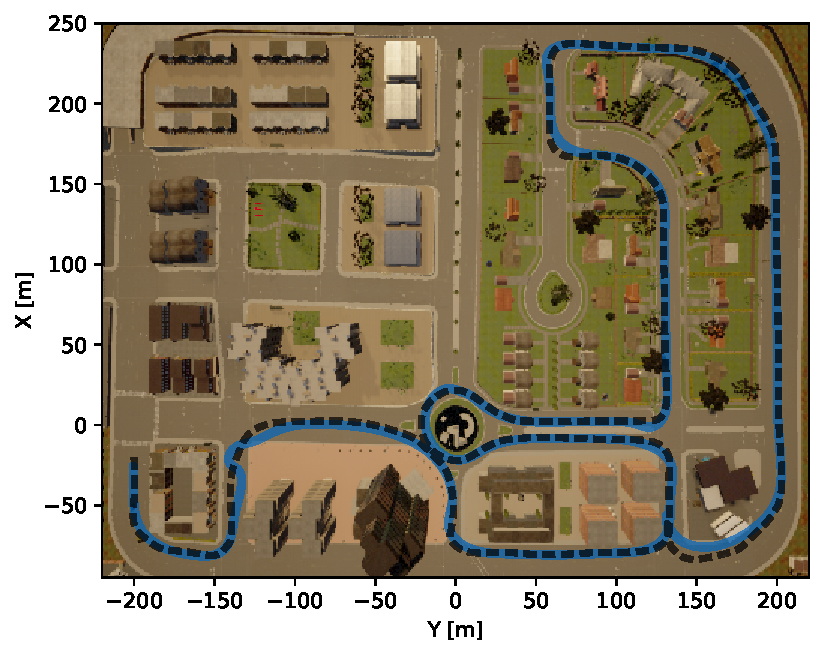
\includegraphics[width=1\textwidth]{images/trajectory_img_h.pdf}
    \caption[Example of a difficult drive trajectory in the CARLA simulator]{Example of a difficult drive trajectory in the CARLA simulator. The full blue line represents the trajectory of the chasing car and the dashed black line represents the trajectory of the pursued car. }\label{f:trajectory}
\end{figure}


We divide the dataset into two equal-sized sets based on difficulty. The first set contains simple drives in which the car was driven slowly and without sudden turning and braking. Any changes such as turns were slow. The average speed in these drives is 35.01 km/h.\par


On the other hand, the second set aims to test the algorithm to its limits. The drives include sudden braking, fast turns as well as cutting corners. Sometimes even drifts were performed. The average speed in these drives is 49.68 km/h with the fastest drive having an average speed of 63.29 km/h. %The average speed distribution of both of these sets are seen in Figure \ref{f:speed_distribution}.


% \begin{figure}[]
%     \centering
%     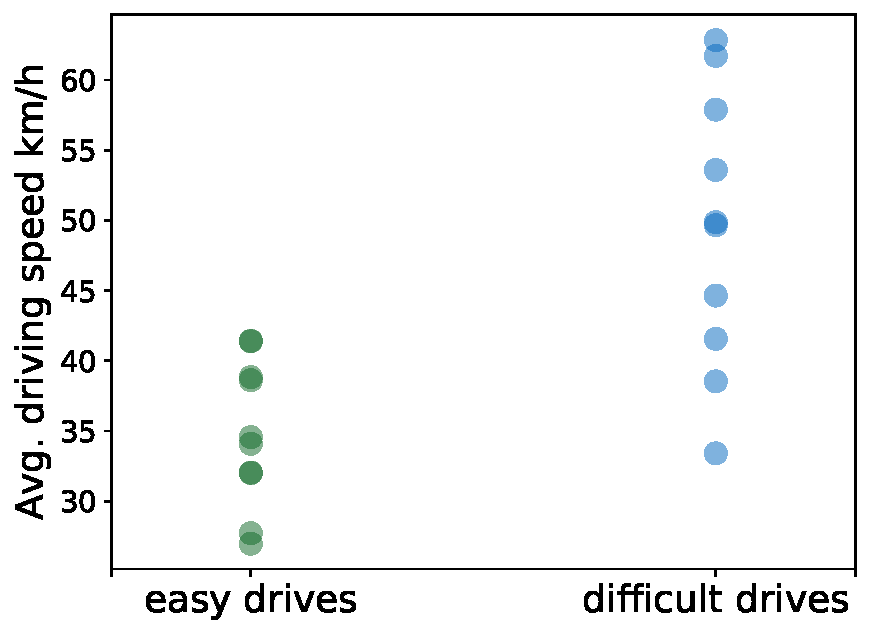
\includegraphics[width=0.7\textwidth]{images/average_speeds.pdf}
    
%     \caption{Average speed distribution of the collected CARLA driving sets}\label{f:speed_distribution}
% \end{figure}



\subsection{Segmentation and Extrapolation Evaluation} \label{s:experiment1}
In the first experiment, we compare different versions of the algorithm. We evaluate the algorithm with its full functionality enabled as described in Section \ref{s:method}, we also test the same algorithm without using coarse image segmentation and finally evaluate the algorithm without the segmentation, and distance and angle extrapolation. We compare these versions on both of the easy and difficult sets described in Section \ref{s:drivingDataset}. We evaluated these versions using 5 indicators. Namely, an average root-mean-square error (RMSE) of the desired distance between the two cars and the actual distance between the two cars. The average mean absolute error (MAE) of the desired and the actual distance. Note that the RMSE and MAE are averaged over the drive trials of the test set. We also measure the average number of crashes per drive. A crash can be a collision with the environment (building for example) or with the pursued car. Furthermore, we measure the average drive completion, which is based on how long the autonomous system was chasing the pursued car. To be specific, at the last position of the chasing car, we calculated the closest point on the chased car path. Then, we calculated the percentage that the part of the path from the beginning point to this point accounts for. Finally, we evaluate the total number of finished drives. We consider the chase to be finished if the drive was at least 95\% completed.\par

\begin{table}[]
\tabcolsep=0.11cm
\begin{tabular}{l|lllll}
\hline
                                      & Finished & Avg. Completion  & Crashes & MAE  & RMSE   \\ \hline
Full Algorithm                         & 10       & 97.48\% & 0.1     & 9.28 & 10.91 \\
W/o Segmentation                    & 10       & 97.41\%          & 0.1     & 9.26 & 10.90 \\
W/o Segm. + Ex. & 9        & 97.03\%          & 0.11    & 9.34 & 11.23 \\ \hline
\end{tabular}
\caption{Comparison of the different algorithm versions on the easy driving set}\label{t:easy_drives}
\end{table}


\begin{table}[]
\tabcolsep=0.11cm
\begin{tabular}{l|lllll}
\hline
                                      & Finished & Avg. Completion & Crashes & MAE   & RMSE   \\ \hline
Full Algorithm                         & 4               & \textbf{63.84\%}         & 1.5     & 14.39 & 18.30    \\
W/o Segmentation                   & 4               & 54.76\%                  & 1.25    & 14.30 & 18.22 \\
W/o Segm. + Ex. & 3               & 53.29\%                  & 1       & 14.49 & 18.89    \\ \hline
\end{tabular}
\caption{Comparison of the different algorithm versions on the difficult driving set}\label{t:difficult_drives}
\end{table}

Table \ref{t:easy_drives} shows results on the easy test set. All three versions of the system performed well with even the simplest version finishing most of the drives. \par
Table \ref{t:difficult_drives} compares the versions using the difficult driving set. We can see, that the full versions of the algorithm performed significantly better than the remaining two versions. It achieved almost 10\% higher average drive completion than the next best-evaluated version. We attribute this to the use of coarse semantic segmentation. Figure \ref{fig:prubehy} depicts experimental results of the full system during a difficult drive shown in Figure \ref{fig:CARLA}.\par

\begin{figure}[]
    \centering
    \subfloat[Distance between the two cars]{{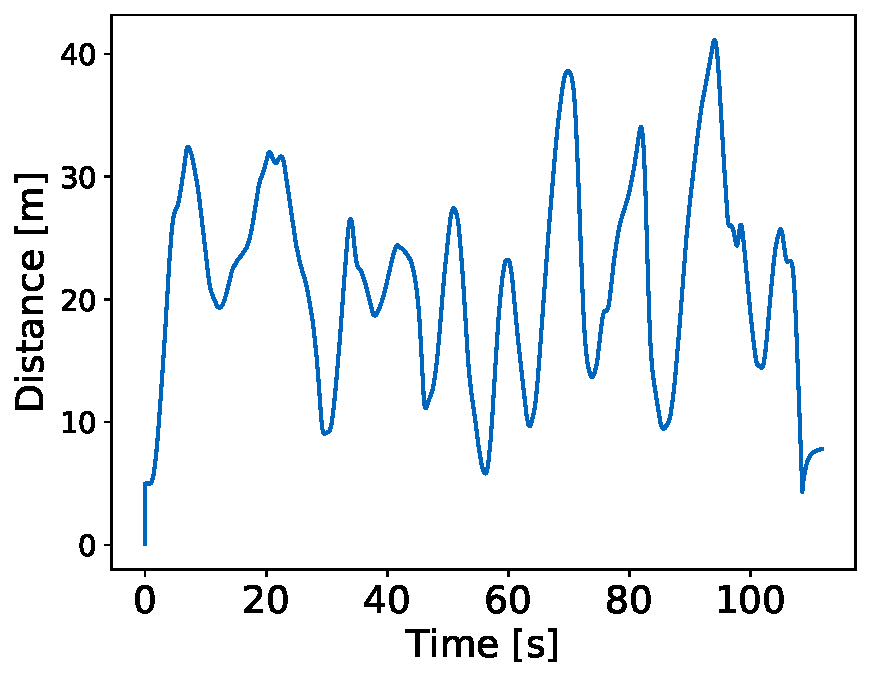
\includegraphics[width=0.46\textwidth]{images/distances.pdf} }}%
    \quad
    \subfloat[Car speed of the two cars]{{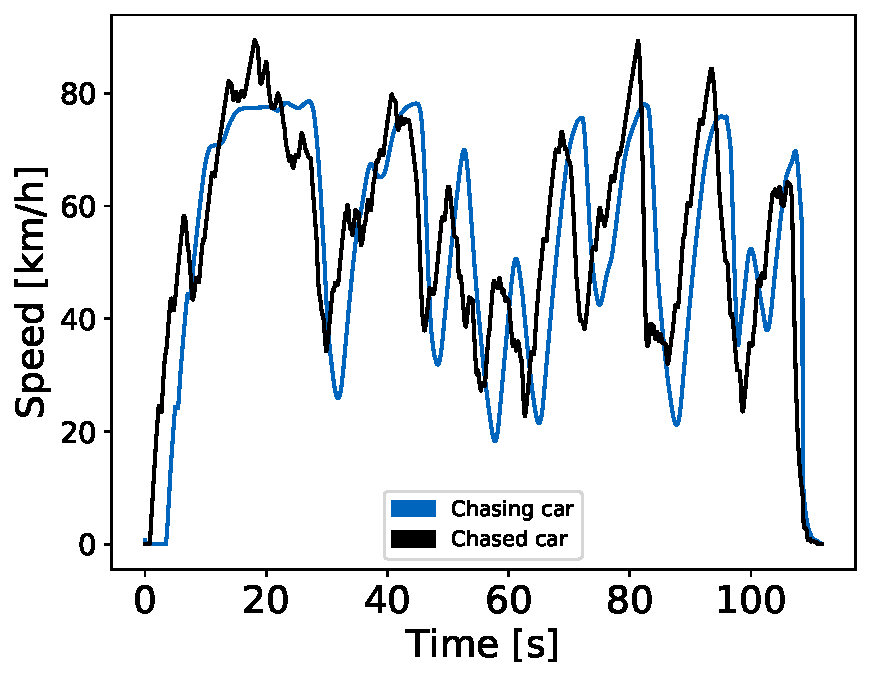
\includegraphics[width=0.46\textwidth]{images/speeds.pdf} }}%
    \quad
    \subfloat[Angle between the two cars]{{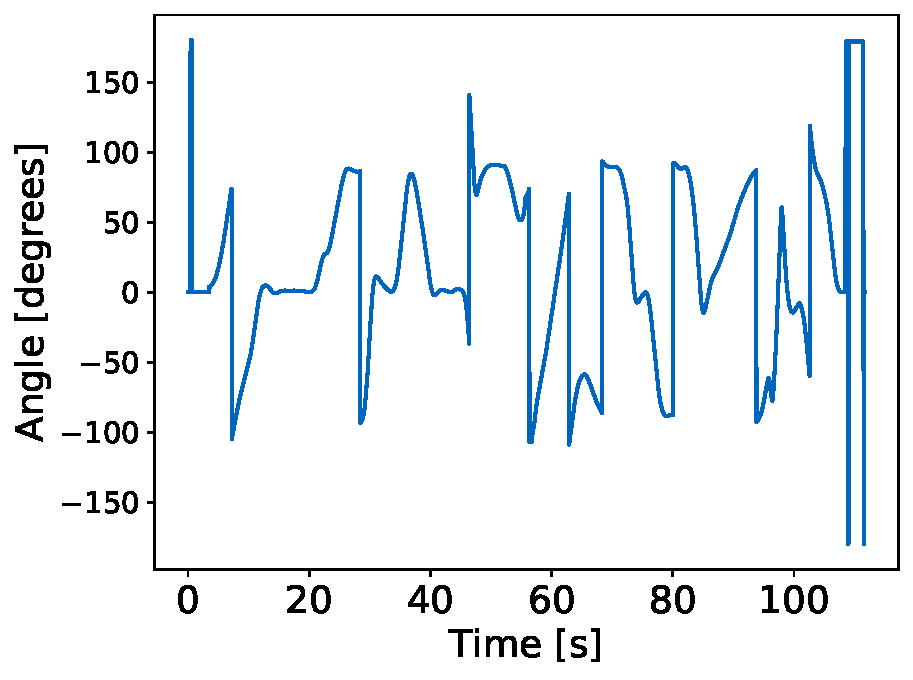
\includegraphics[width=0.46\textwidth]{images/angles.pdf} }}%
    \quad
    \subfloat[Yaw rate of the two cars]{{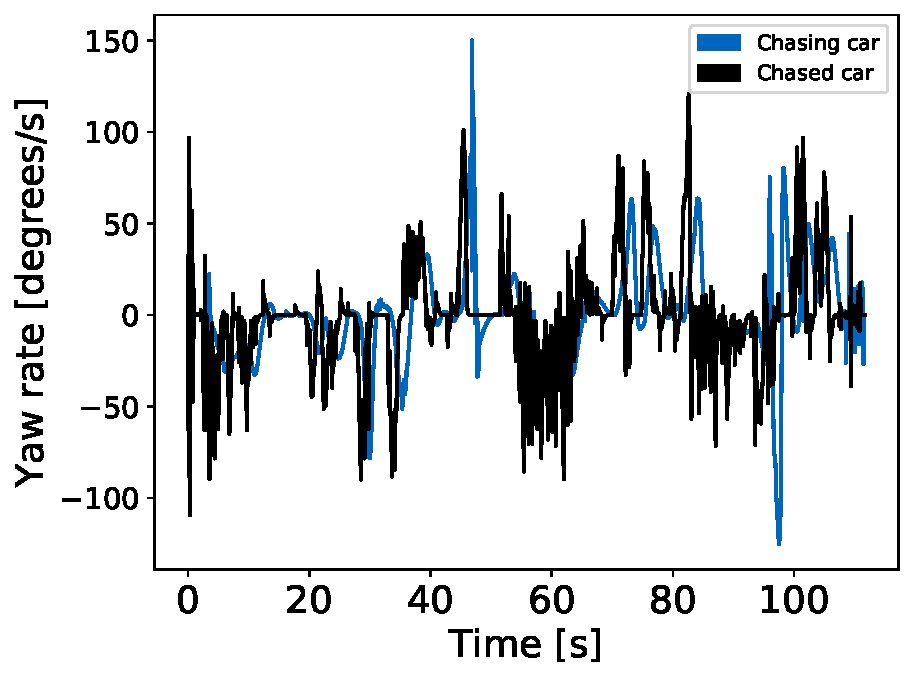
\includegraphics[width=0.46\textwidth]{images/yaw_rate.pdf} }}%
    \caption{Different metrics of the car chase shown in Figure \ref{fig:CARLA} in time.}%
    \label{fig:prubehy}
\end{figure}




\subsection{Impact of the Detector Quality on Chasing Success}
As we can see in Table \ref{tab:detection} the recall of the detector is significantly lower than its precision. Therefore, in this experiment, we investigate the effects of detectors recall on the ability of the autonomous driving system to chase another vehicle. The failed detections had a uniform distribution over the frames of the sequence. Furthermore, we investigate how each of the three versions of the system copes with different detection recall levels. Figure \ref{f:detection_recall} plots the average drive completion (of the 20 drives) described in Section \ref{s:experiment1} against the detection recall. \par


\begin{figure}[]
    \centering
    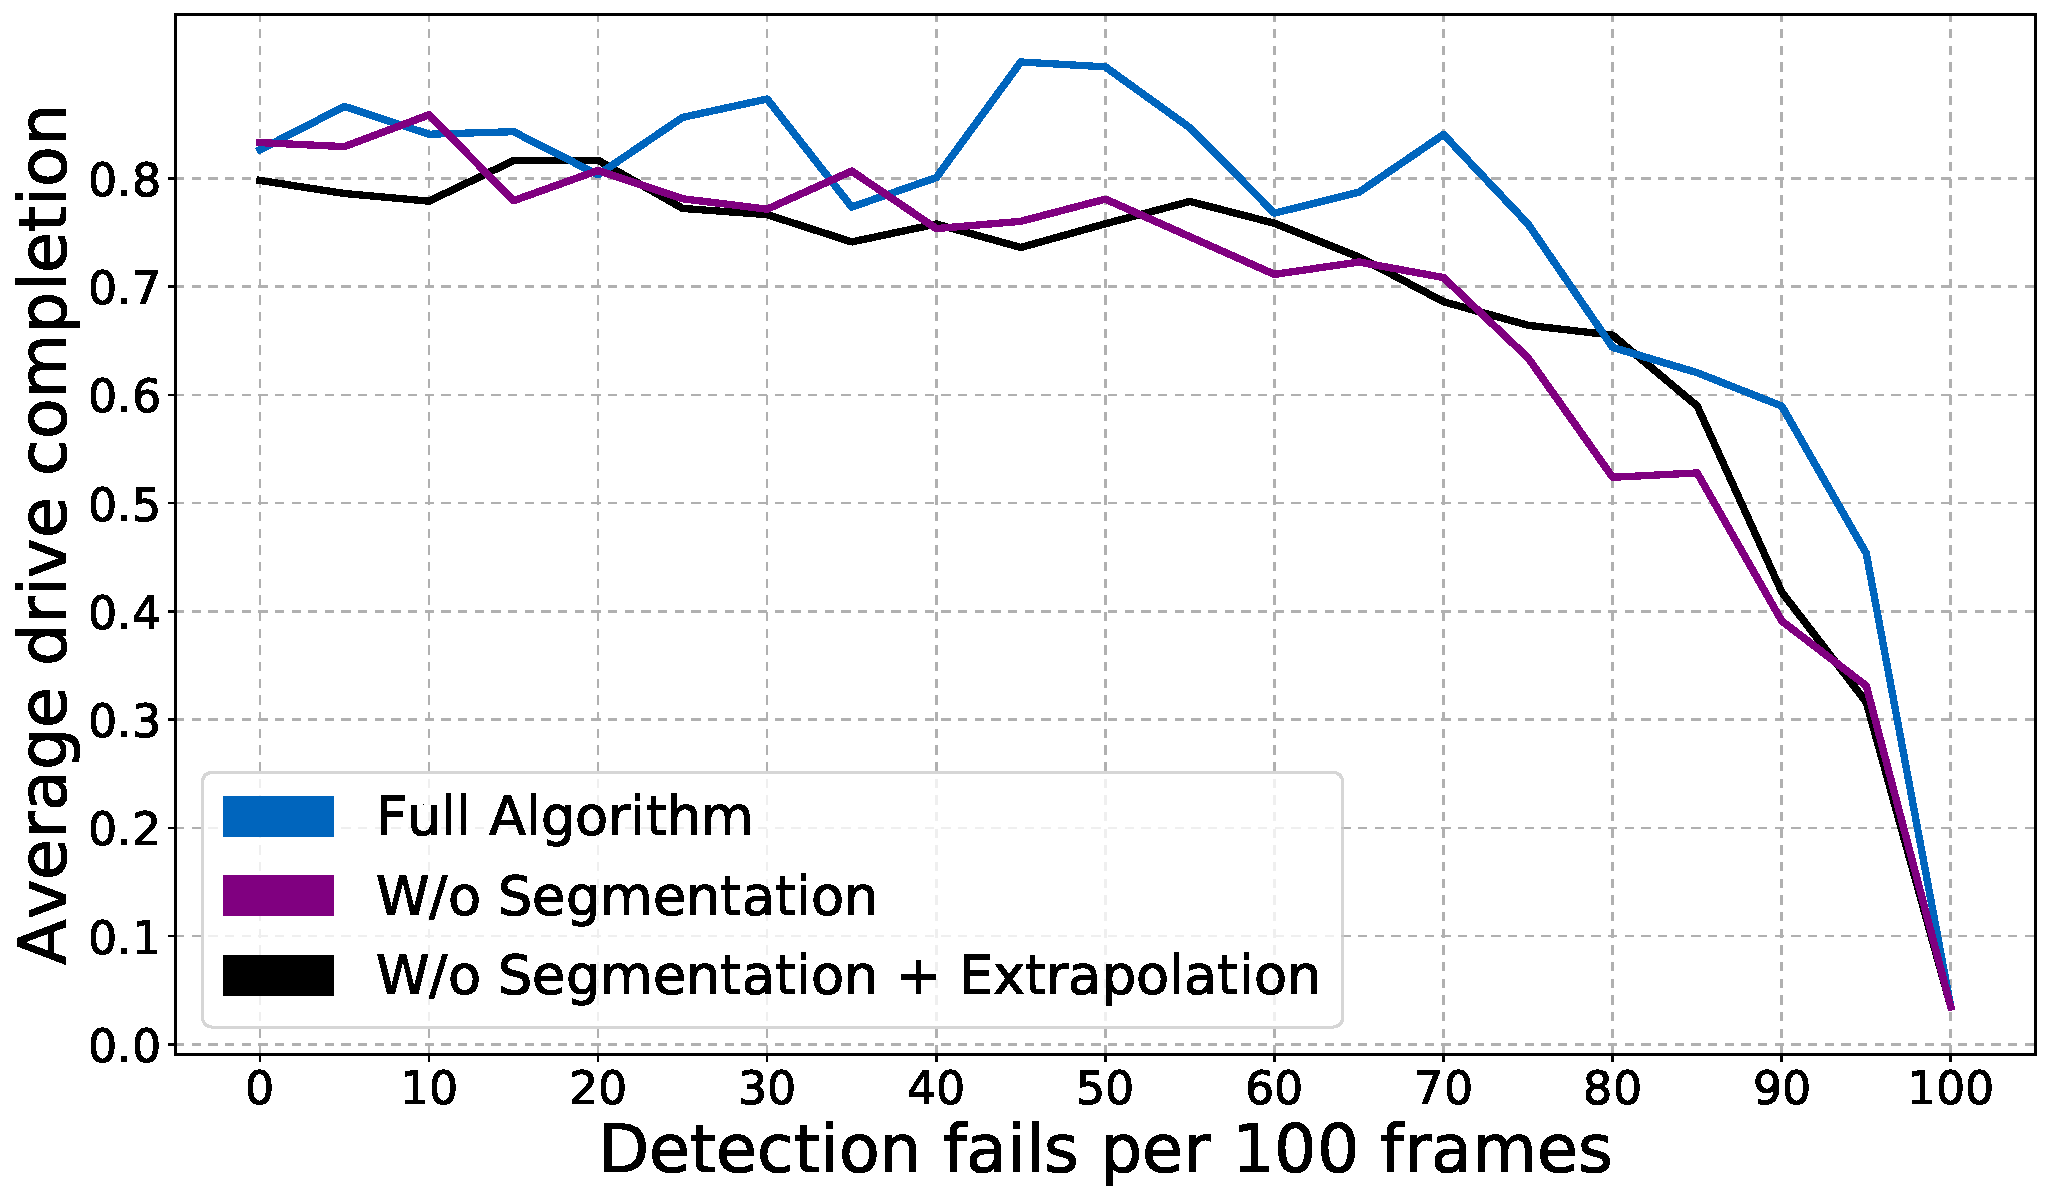
\includegraphics[width=1\textwidth]{images/recall_chart7.pdf}
    
    \caption{Average drive completion plotted against detection recall. All drives included}\label{f:detection_recall}
\end{figure}

From Figure \ref{f:detection_recall} we can see, that the average drive completion steadily declines with decreasing detection recall and the system starts to fail once the detection recall is at 25\%. Out of the three versions of the algorithm, the full version which uses coarse semantic segmentation and angle and distance extrapolation of the pursued car performs the best. It maintains above 80\% drive completion until the detection recall gets below 25\%. We attribute this achievement to the use of coarse semantic segmentation. We base this assumption on the fact, that the version of the system that uses extrapolation but does not use segmentation performs similarly to the version which does not use extrapolation nor the segmentation. \par

Figure \ref{f:detection_recall_difficult} plots the average drive completion on the difficult driving set against detection recall. On this driving set, the full version of the algorithm performs even more significantly better than the other two versions. When the recall is at 60\% or lower, the average drive completion of the full version is almost 20\% higher than the average drive completion of the remaining two versions.

\begin{figure}[]
    \centering
    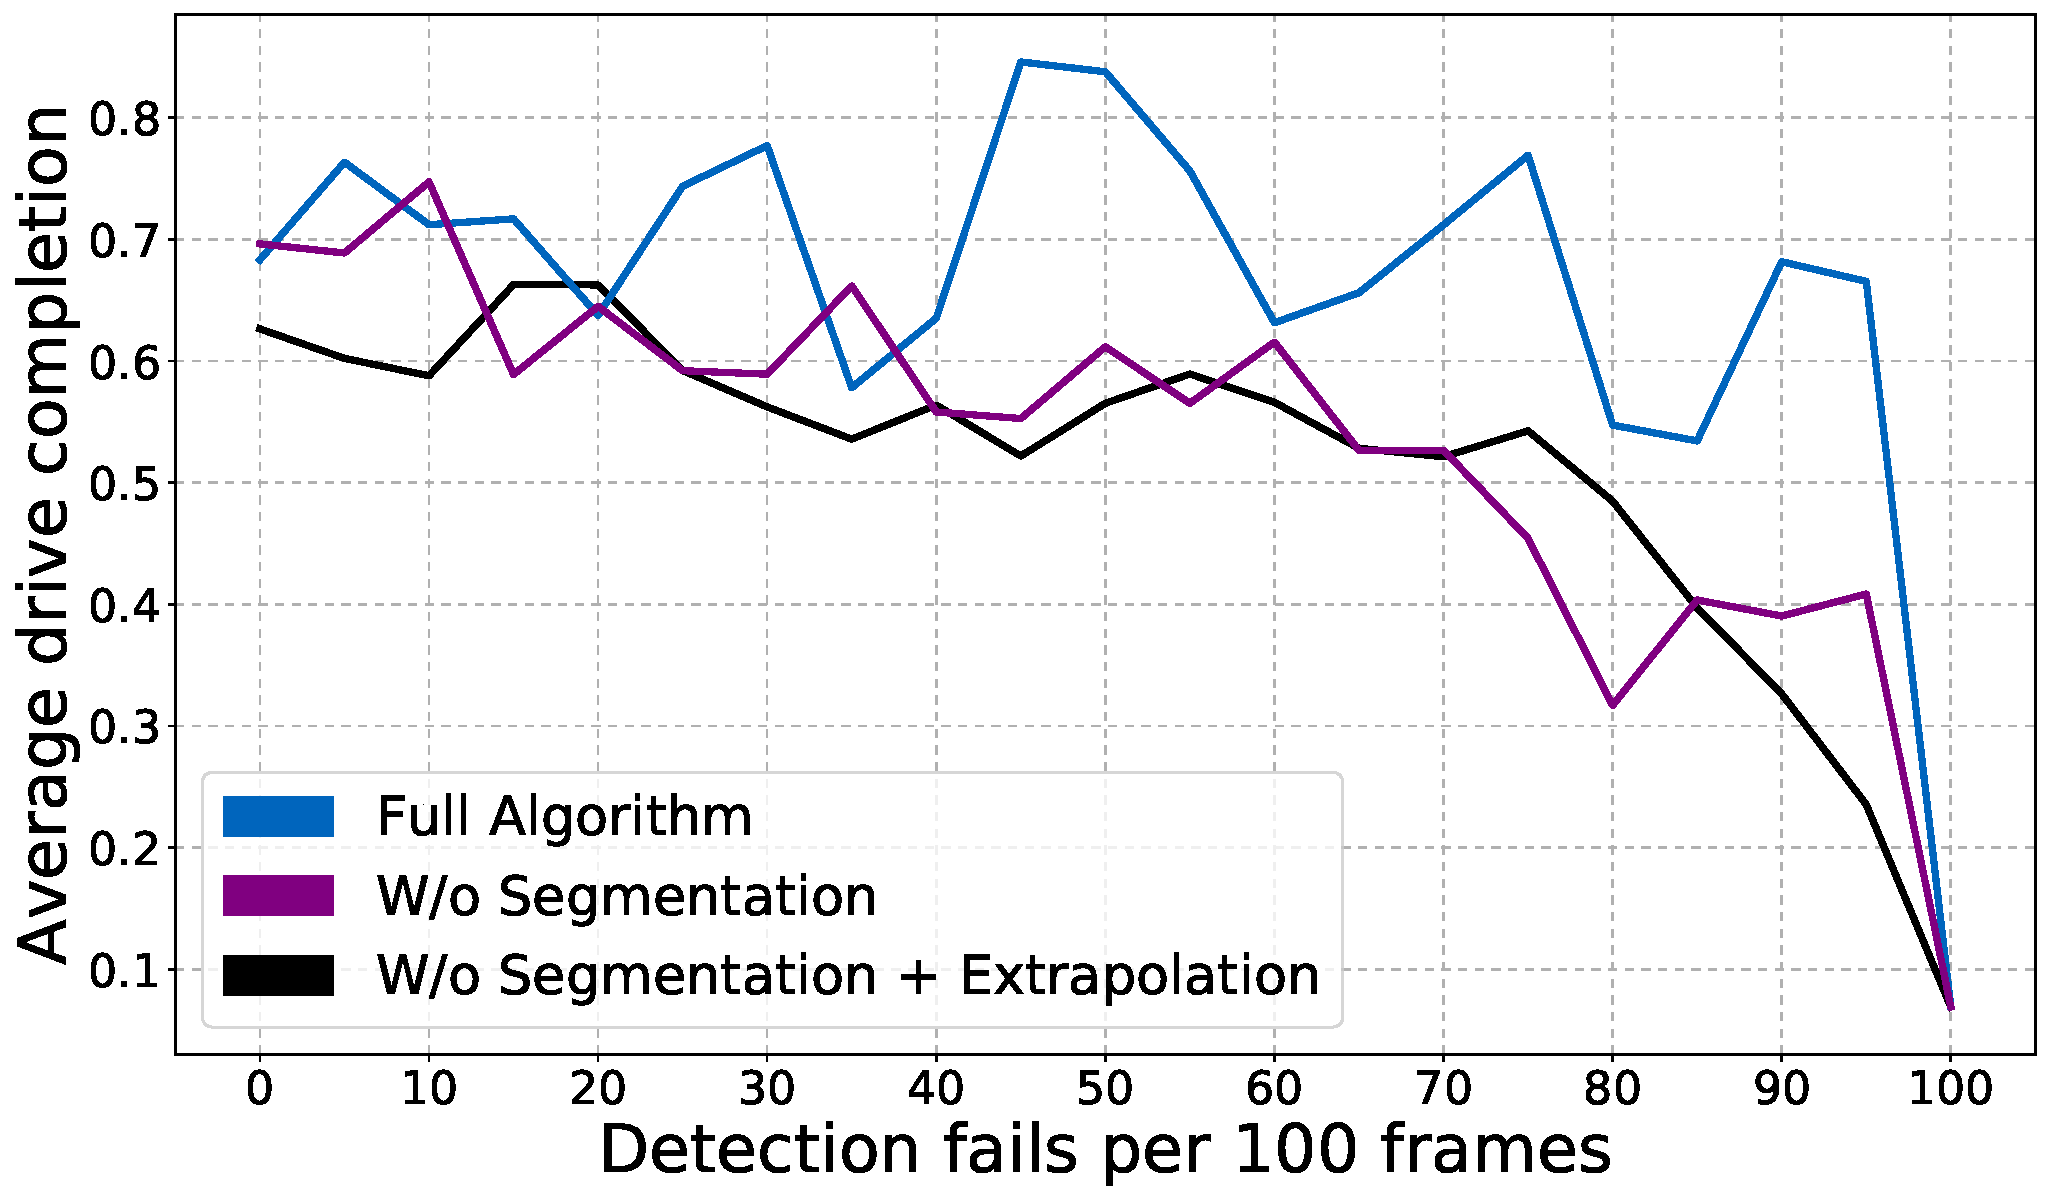
\includegraphics[width=1\textwidth]{images/recall_chart7_difficult.pdf}
    
    \caption{Average drive completion plotted against detection recall. Only difficult drives included}\label{f:detection_recall_difficult}
\end{figure}


\subsection{Qualitative results}
While performing the experiments, we saw that the use of coarse semantic segmentation allowed the system to stay longer on the road in situations when the pursued car was not detected for a prolonged period. For example, when the pursued car drove behind a building, both versions of the algorithm that use extrapolation correctly predicted the position of the pursued car. However, the algorithm that did not use segmentation drove straight into the building and collided as it did not have any information about its surrounding environment. Only the full version of the algorithm drove around the building and continued the chase.


%\footnote{Available at \href{https://github.com/JahodaPaul/autonomous-car-chase}{https://github.com/JahodaPaul/autonomous-car-chase}}
\section{Real Tests}
\subsection{Vehicle Detection}
\subsubsection{Dataset} \label{s:detection_dataset}
In order to train and evaluate an object detector capable of predicting a 2D bounding box around the chased RC car in an image, a dataset was needed. The collected dataset \cite{my_github} consists of \textbf{460} manually annotated images. All image annotations are in the PASCAL VOC data format introduced in the PASCAL Visual Object Classes Challenge \cite{pascal-voc}. Each image has its annotation that contains pixel coordinates of the bounding box corners for each object in the image. In our dataset, a single object per image is present -- the chased RC car. The data were collected from multiple locations around Czechia, on various surfaces, and also under different lighting conditions. The majority of images were collected by the ZED Stereo camera attached to the chasing RC car. Around 5\% of the collected images were taken with smartphone Xiaomi Mi 8. A few images from the dataset are shown in Figure \ref{f:dataset_detection}.

\begin{figure}[]
    \centering
    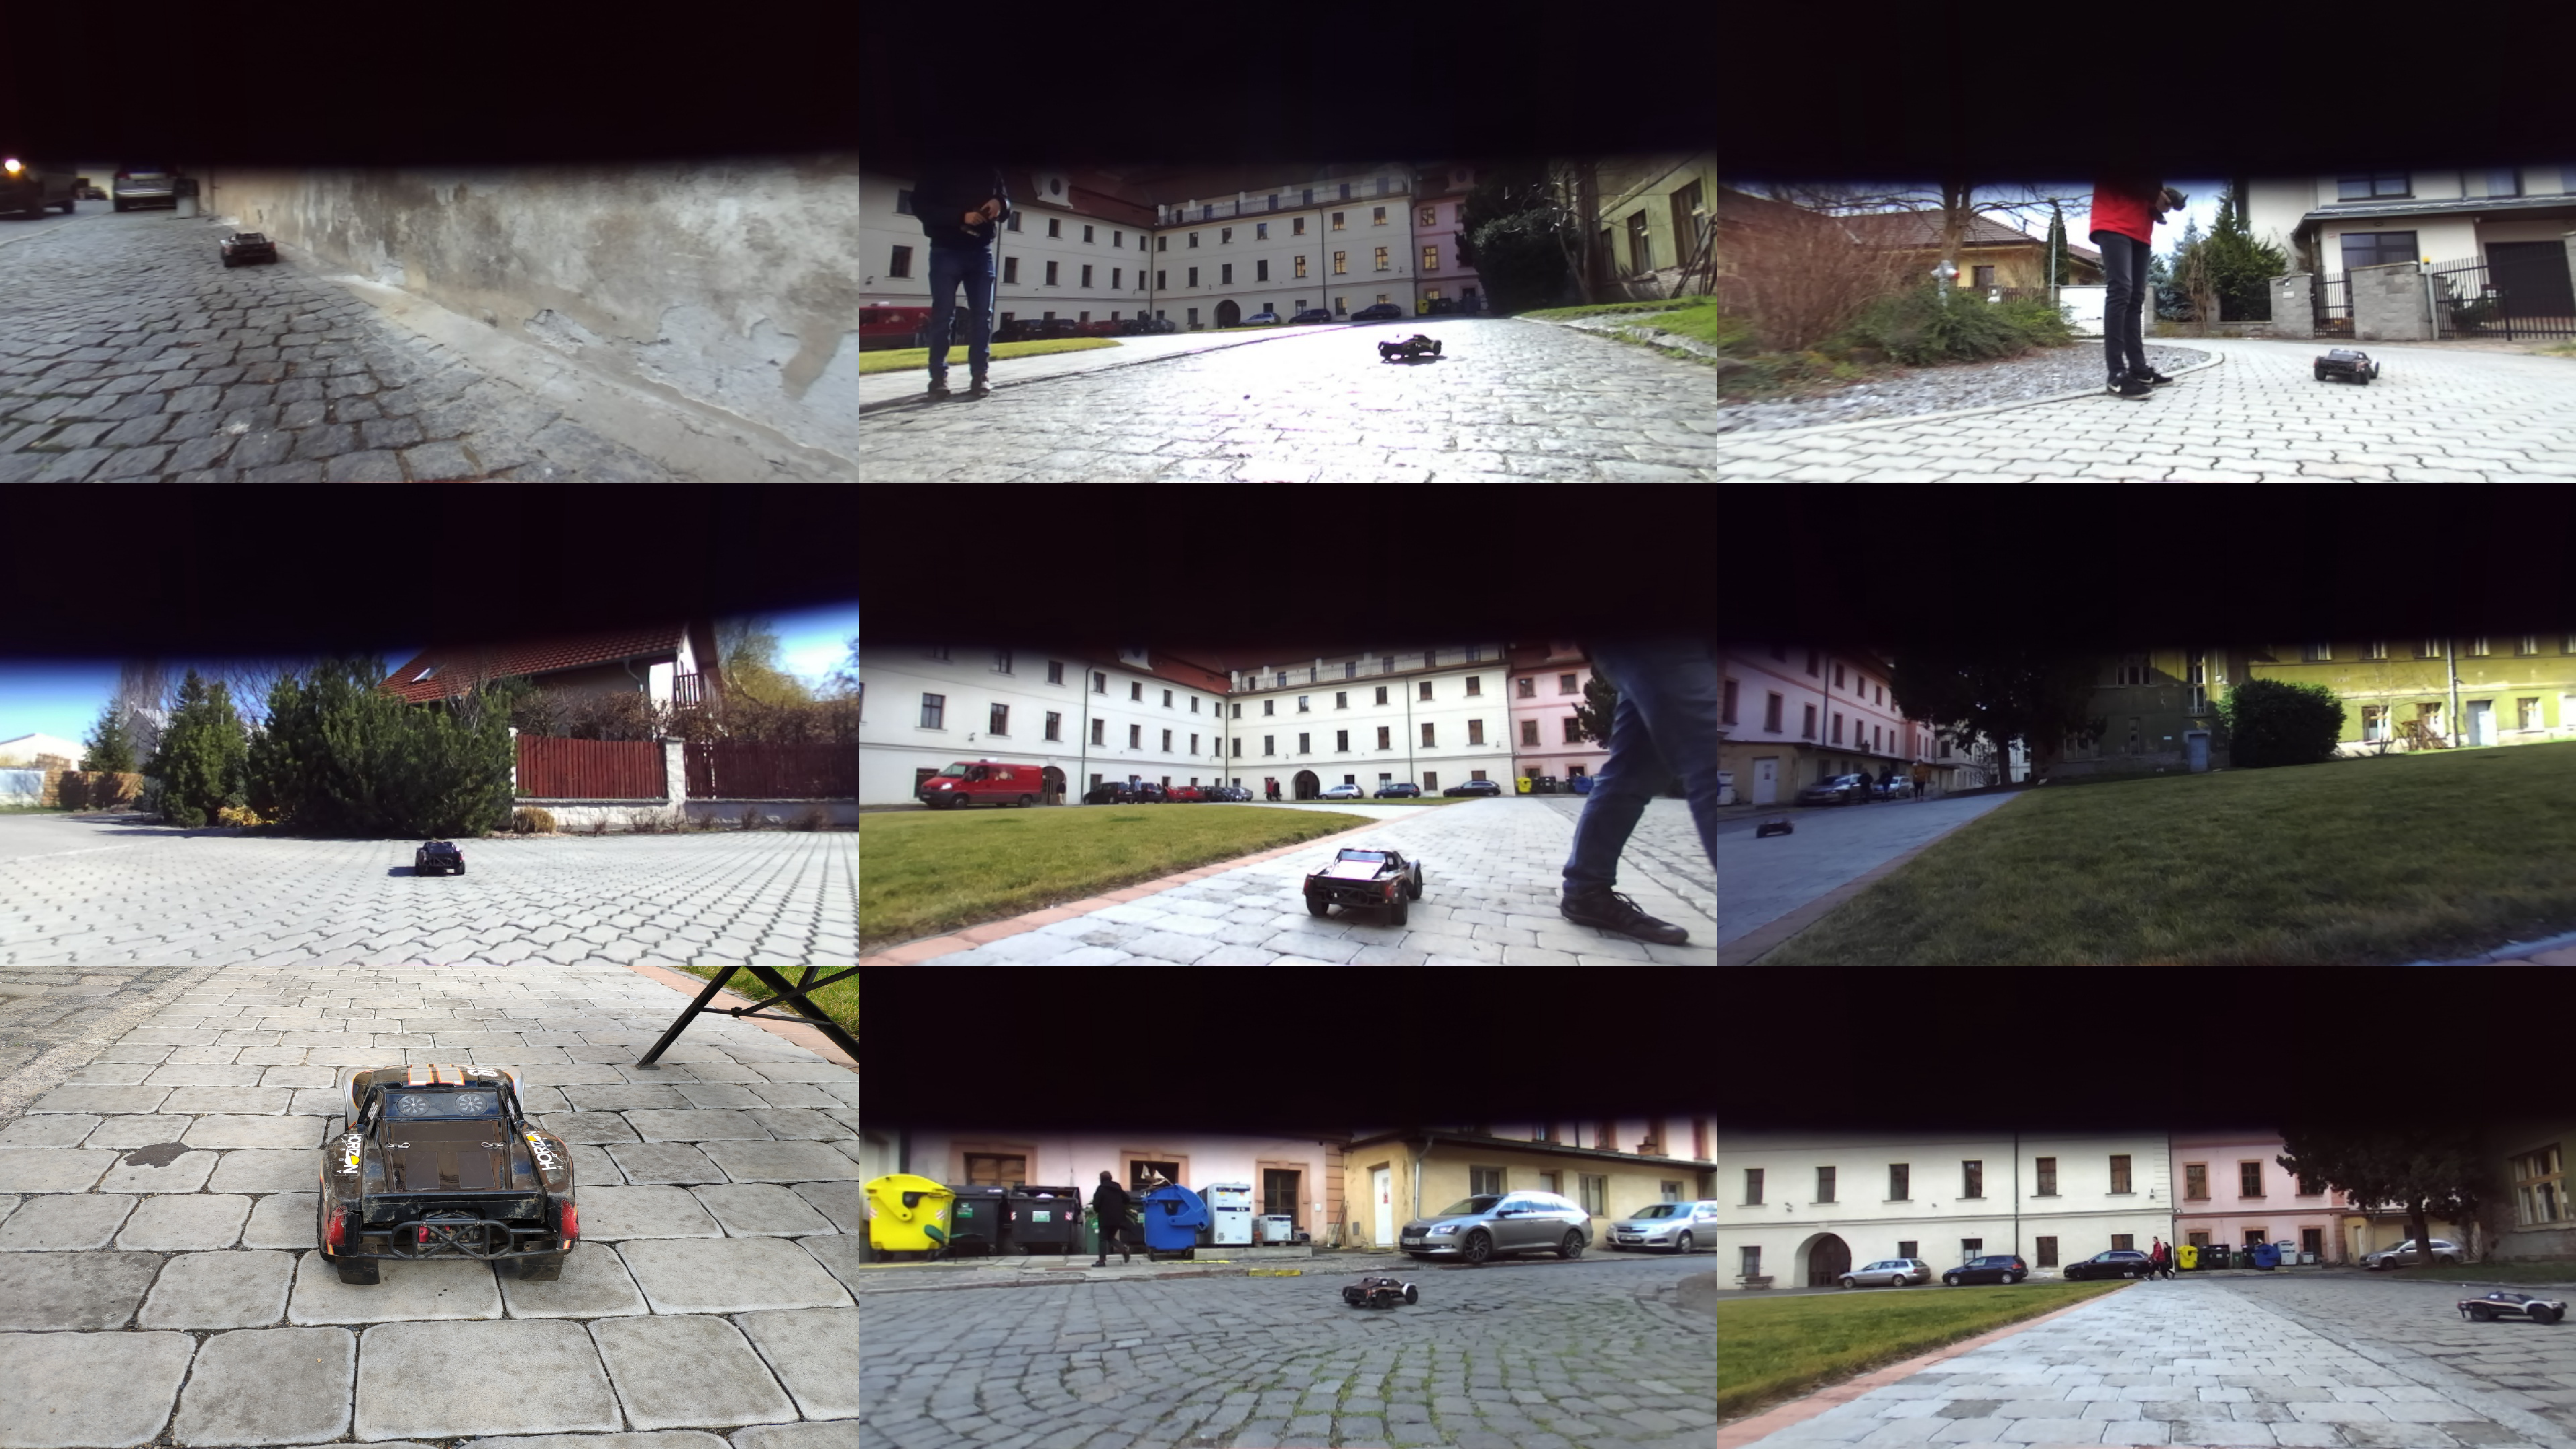
\includegraphics[width=1\textwidth]{images/dataset_collage.pdf}
    
    \caption{Detection dataset. Overview of the environment variability present in the dataset}\label{f:dataset_detection}
\end{figure}


\subsubsection{Detection Results}
The collected dataset was split into three sets. The majority of 80\% of the images were randomly selected into a training set, 10\% were randomly selected into a validation set and the remaining images were used as a test set. To evaluate the model, we calculated multiple statistics -- recall, precision, XY loss, and WH loss. To explain recall and precision we need to first define IoU (Intersection over union). IoU measures how much the predicted bounding box overlaps with the ground truth (annotated bounding box). It is defined as 
\begin{equation}IoU = \cfrac{\textrm{Area of overlap}}{\textrm{Area of union}}\end{equation}

%When calculating precision and recall, we say that the prediction is either true positive or false positive when IoU is greater than $0.5$.
%Finally if no ground truth object of some class $c$ is present in the image and no bounding box for class $c$ was predicted we classify it as ($tn$).

We say that the prediction is true positive ($tp$) when IoU between the predicted bounding box and the ground truth bounding box is greater than $0.5$. We say that it is false positive ($fp$) if it is less or equal to $0.5$. When a ground truth bounding box is present in the image and the model failed to detect the object, we classify it as false negative ($fn$). Finally, we define recall as $recall=\frac{tp}{tp+fn}$ and precision as $precision=\frac{tp}{tp+fp}$. We calculate XY loss as a mean squared error (MSE) between the center of the predicted bounding box and the center of the ground truth bounding box. WH loss, on the other hand, is the difference between width and height of the predicted bounding box and the ground truth bounding box. When calculating both of these values, coordinates and image dimensions have been scaled to the [0, 1] range. \par

During training, the model with the smallest sum of the WH and XY losses on the validation dataset has been selected. The evaluation of the detector on the test set is shown in Table \ref{tab:detection}. Results indicate that the pre-trained model detects the chased car accurately. This is achieved with only a few hundred training examples. Examples of the detection, together with angle and distance estimates are shown in Figure \ref{f:detection_images}. 

\begin{table}[]
\begin{tabular}{l|llll}
\hline
            & Precision & Recall & XY loss & WH loss \\ \hline
Test set & 99.8\%    & 97.7\% & 0.066   & 0.227   \\ \hline
\end{tabular}
\caption{Evaluation of the detector on a test set}\label{tab:detection}
\end{table}



\begin{figure}[]
    \centering
    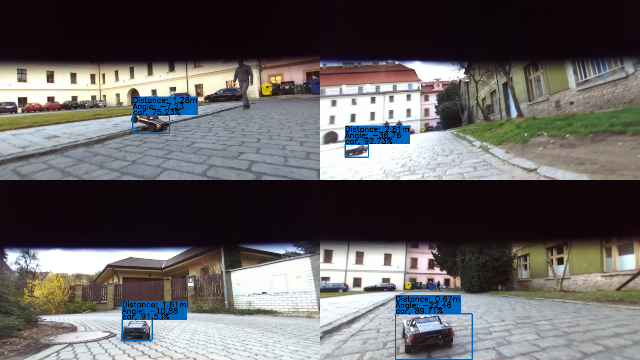
\includegraphics[width=1\textwidth]{images/detection_collage.pdf}
    
    \caption[Detection bounding boxes, distance, and angle estimation performed on images from the RC car camera]{Detection bounding boxes, distance, and angle estimation performed on images from the RC car camera. The images are part of the test split of the collected dataset}\label{f:detection_images}
\end{figure}



\subsection{Segmentation Results}
To train and evaluate the coarse semantic segmentation part of the dual-task neural network, we have annotated the collected detection dataset presented in Section \ref{s:detection_dataset}. As explained in Section \ref{s:Image_Segmentation}, each image is segmented into a $10\times 10$ grid of cells. Therefore, we treat this as a classification problem, where the network performs 100 classifications per image. We report, that the neural network achieved 94.4\% classification accuracy on the test set.

\begin{figure}[h]
    \centering
    \subfloat[Class distribution]{{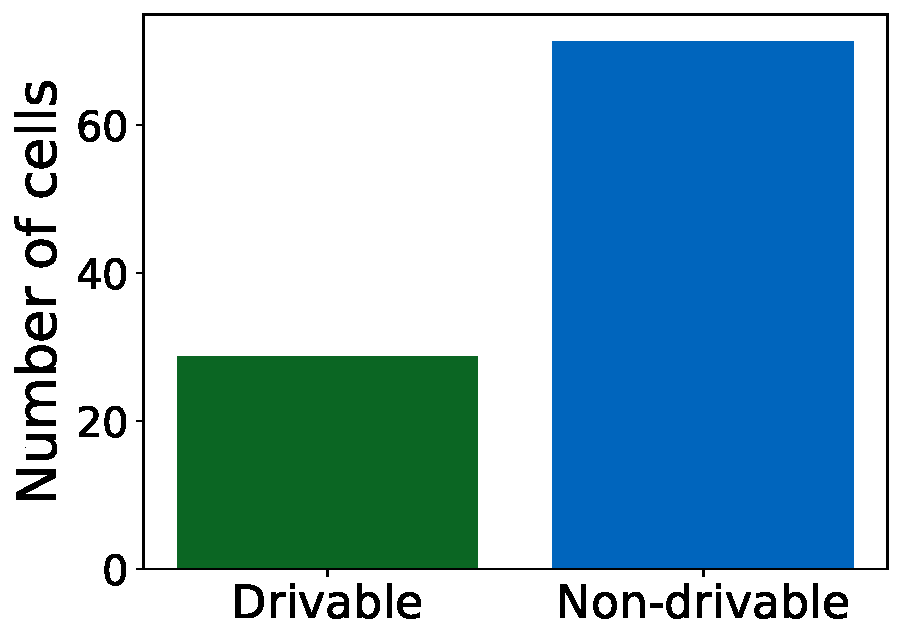
\includegraphics[width=0.46\textwidth]{images/bar_chart_drivable.pdf} }}%
    \quad
    \subfloat[Confusion matrix. Value P represent Drivable surface while N represents the non-drivable surface
]{{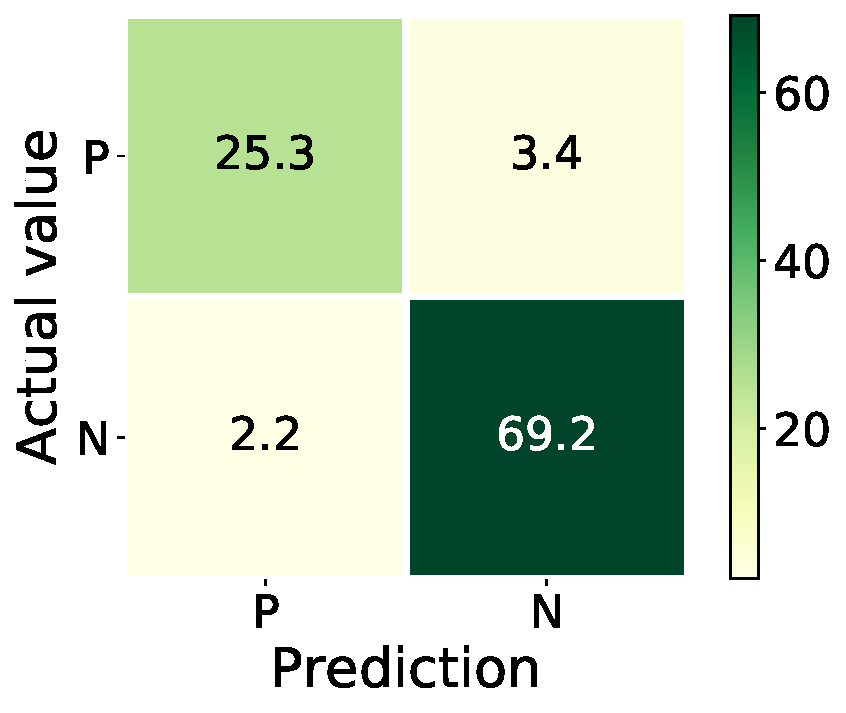
\includegraphics[width=0.46\textwidth]{images/confusion_matrix.pdf} }}%
    \caption[Confusion matrix of the coarse segmentation predictions and class distribution of the test set]{Confusion matrix of the coarse segmentation predictions and class distribution of the test set. The numbers represent the number of instances per image, i.e., out of 100 cells in a single image}
    \label{fig:segmentation_results}%
\end{figure}



\subsection{Test Drive Using RC Cars}
\subsubsection{RC Cars Description}
\paragraph{Chasing RC car}
For the deployment of our autonomous chasing algorithm, a subscale vehicle platform called Toyota Mini (ToMi) was used \cite{tomi_Cech2020}. The platform is built around a large 1:5 scale RC car ``Losi Desert Buggy XL-E 4WD'' \footnote{\href{http://www.losi.com/Products/Default.aspx?ProdID=LOS05012T2}{http://www.losi.com/Products/Default.aspx?ProdID=LOS05012T2}}. This electrically powered car has 0.9 x 0.5 meters length and width dimensions with reported maximal speed of up to 80km/h. The platform has a Raspberry Pi with a Navio-board\footnote{\href{https://emlid.com/navio/}{https://emlid.com/navio/}} that generates pulse width modulation (PWM) signals for the throttle and steering to the servomotor. It is also equipped with a ZED stereo camera\footnote{\href{https://www.stereolabs.com/zed/}{https://www.stereolabs.com/zed/}} for taking color images, NVIDIA Jetson AGX Xavier graphics card\footnote{\href{https://www.nvidia.com/en-us/autonomous-machines/embedded-systems/jetson-agx-xavier/}{https://www.nvidia.com/en-us/autonomous-machines/embedded-systems/jetson-agx-xavier/}} for image processing and neural network inference. Finally, it is equipped with SSD to provide additional storage, GPS, and IMU. \par
The whole simplified process flow is as follows. First, an image is taken by a camera, which then goes to the graphics card where it is analyzed by our algorithm. Then, based on the image analysis, both steer and throttle values are updated. These values are transmitted from the graphics card to the Raspberry Pi which then sends a signal to the servomotor that actuates the vehicle.

\paragraph{Chased RC car}
The RC car used as the chased vehicle is a 1:10 scale ``Losi XXX-SCT Brushless RTR''\footnote{\href{http://www.losi.com/Products/Default.aspx?ProdID=LOS03002}{http://www.losi.com/Products/Default.aspx?ProdID=LOS03002}}. This electrically powered car has 0.55 x 0.29 meters length and width dimensions with reported maximal speed of up to 55 km/h. Both vehicles are shown in Figure \ref{fig:rc_cars}.

\begin{figure}[]
    \centering
    \subfloat[Inside of the chasing RC car]{{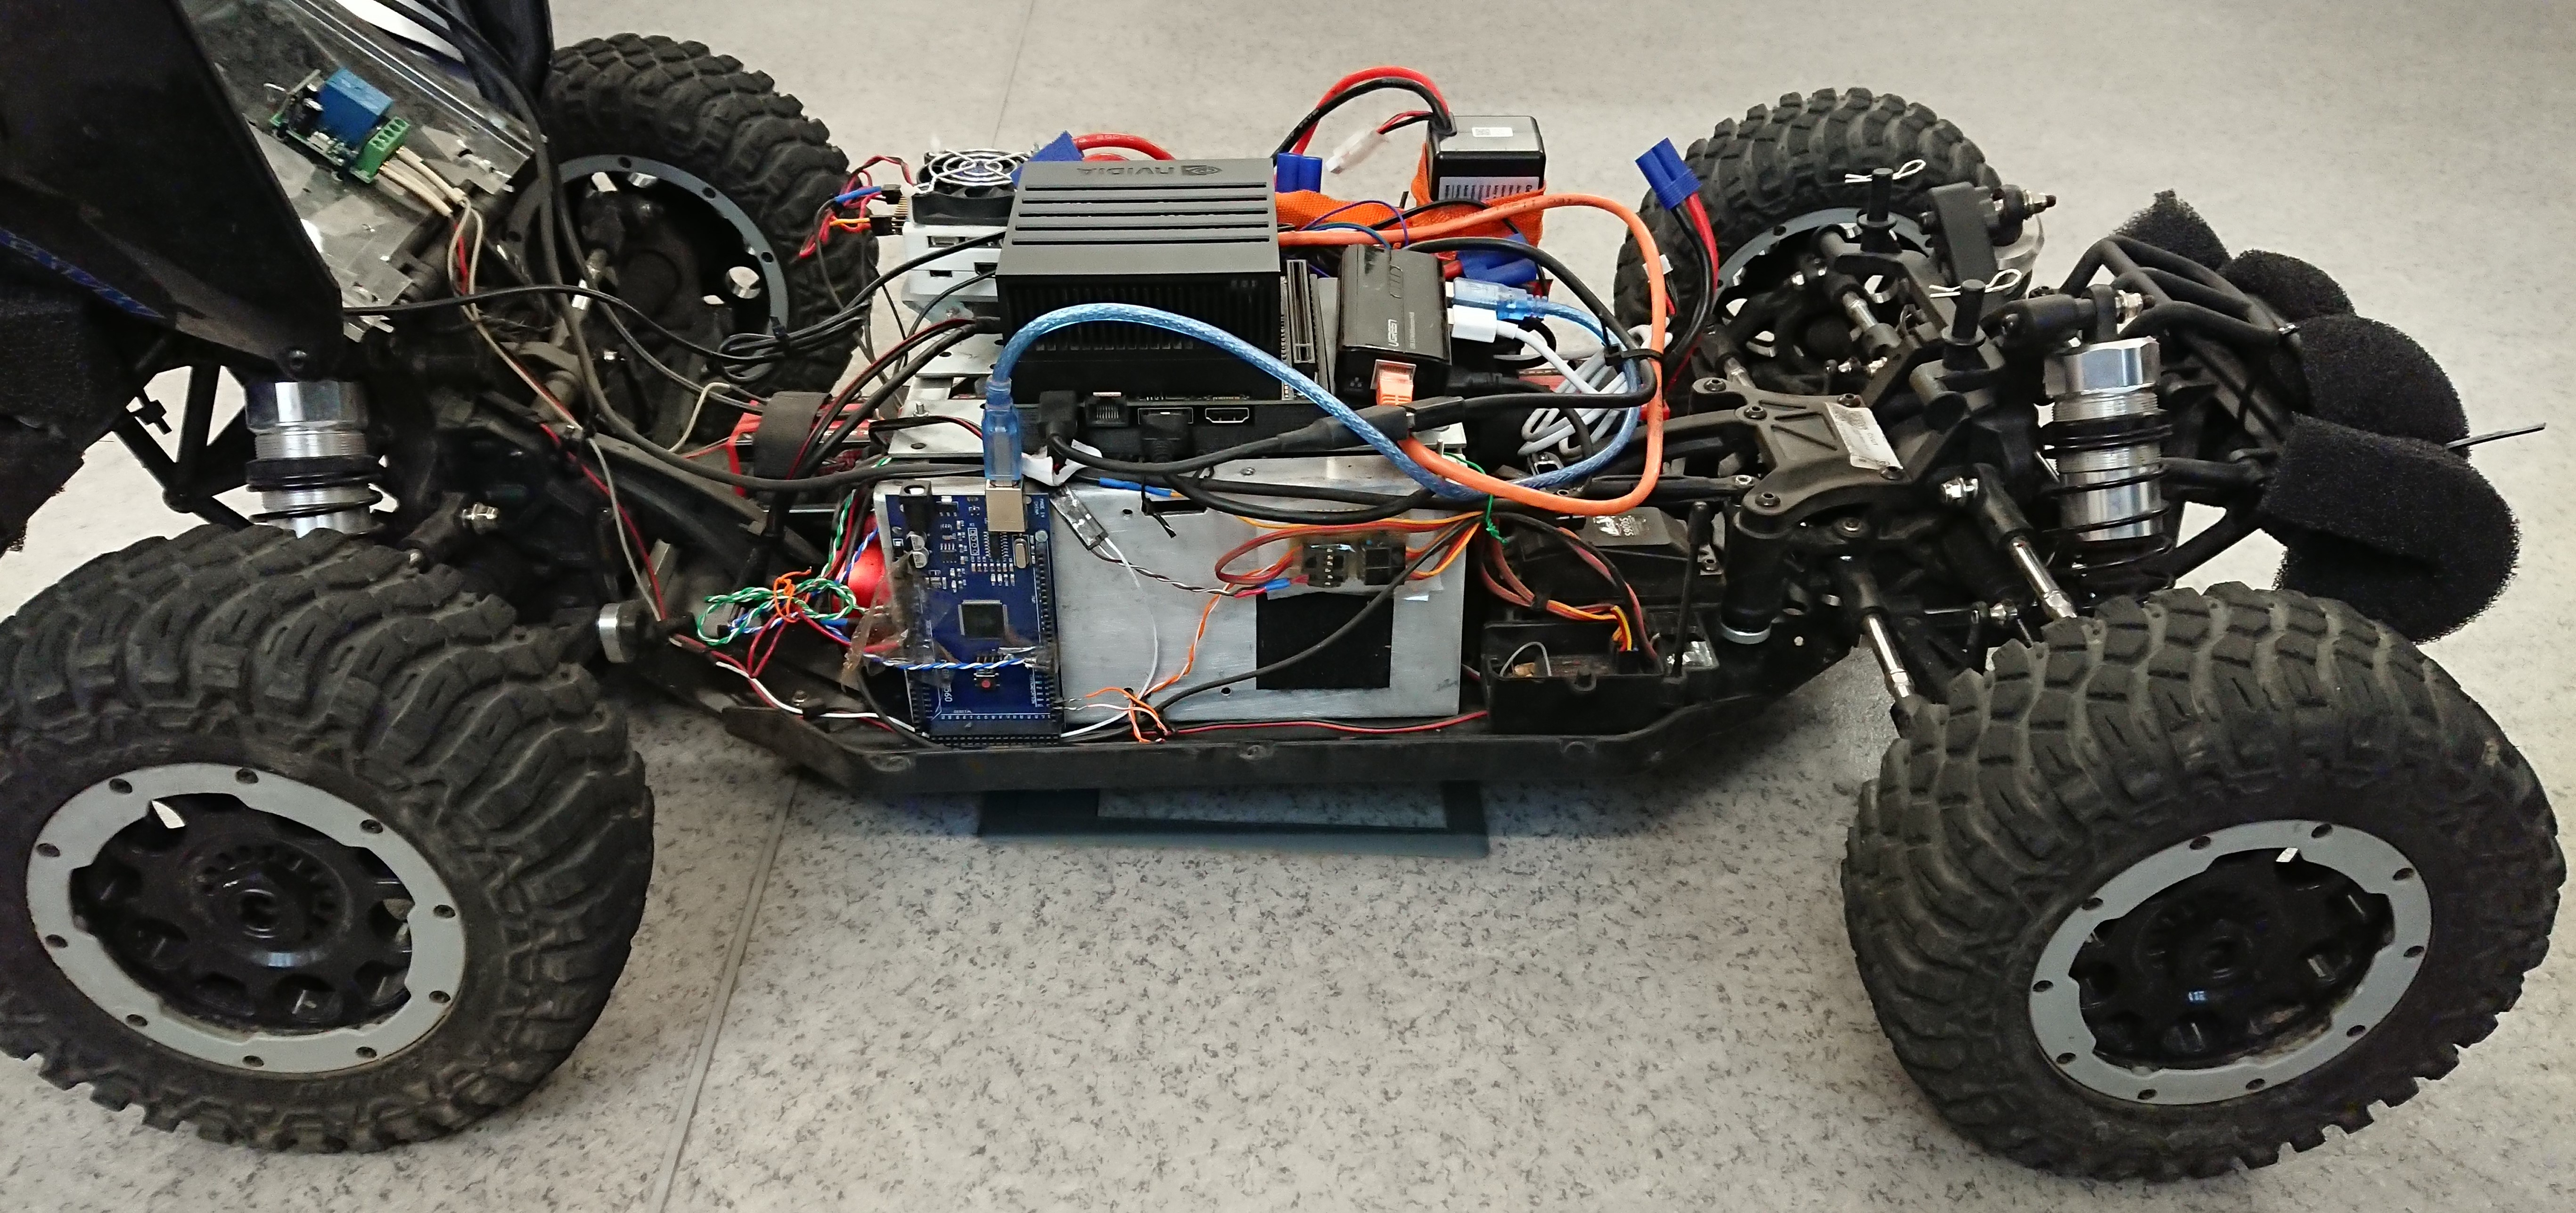
\includegraphics[height=3.7cm]{images/inside.jpg} }}%
    \qquad
    \subfloat[Chasing RC in the back and the chased RC car in the front]{{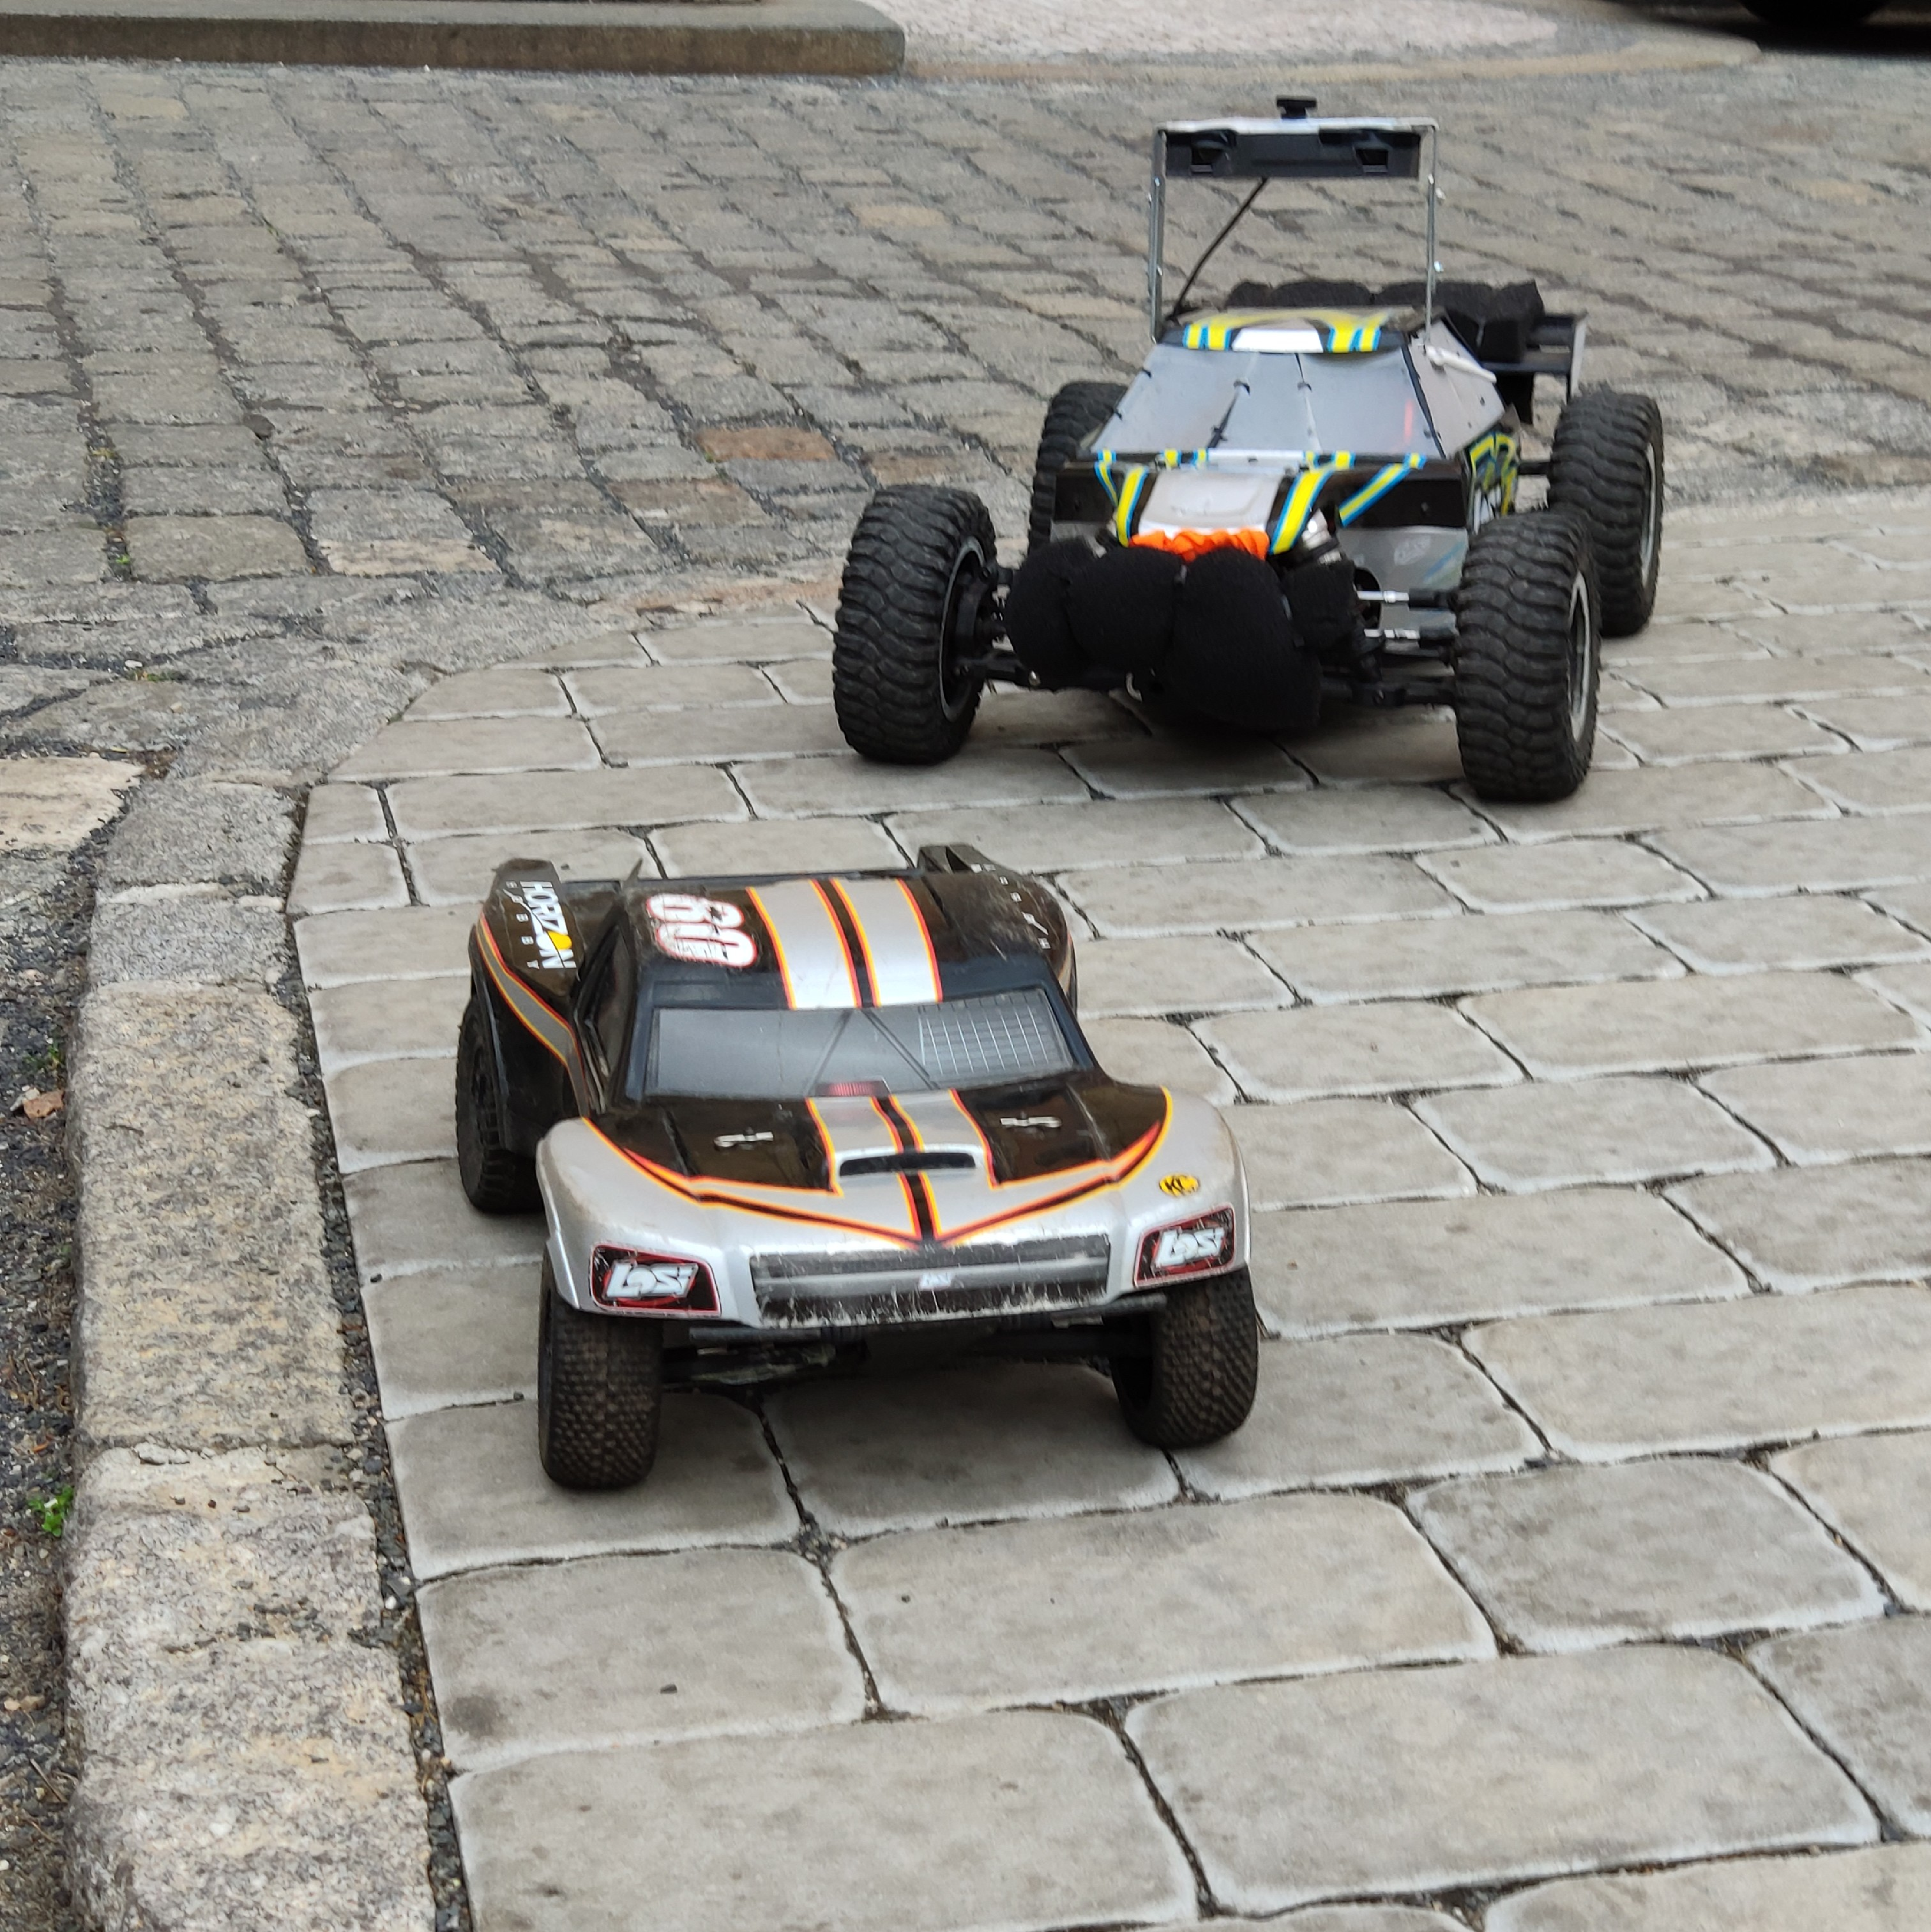
\includegraphics[height=3.7cm]{images/rc_cars.pdf} }}%
    \caption{The hardware inside of the autonomous chasing RC car on the left and both RC cars used for testing on the right}%
    \label{fig:rc_cars}%
\end{figure}

%\begin{figure}[h!]
%\centering
%\begin{subfigure}{.5\textwidth}
%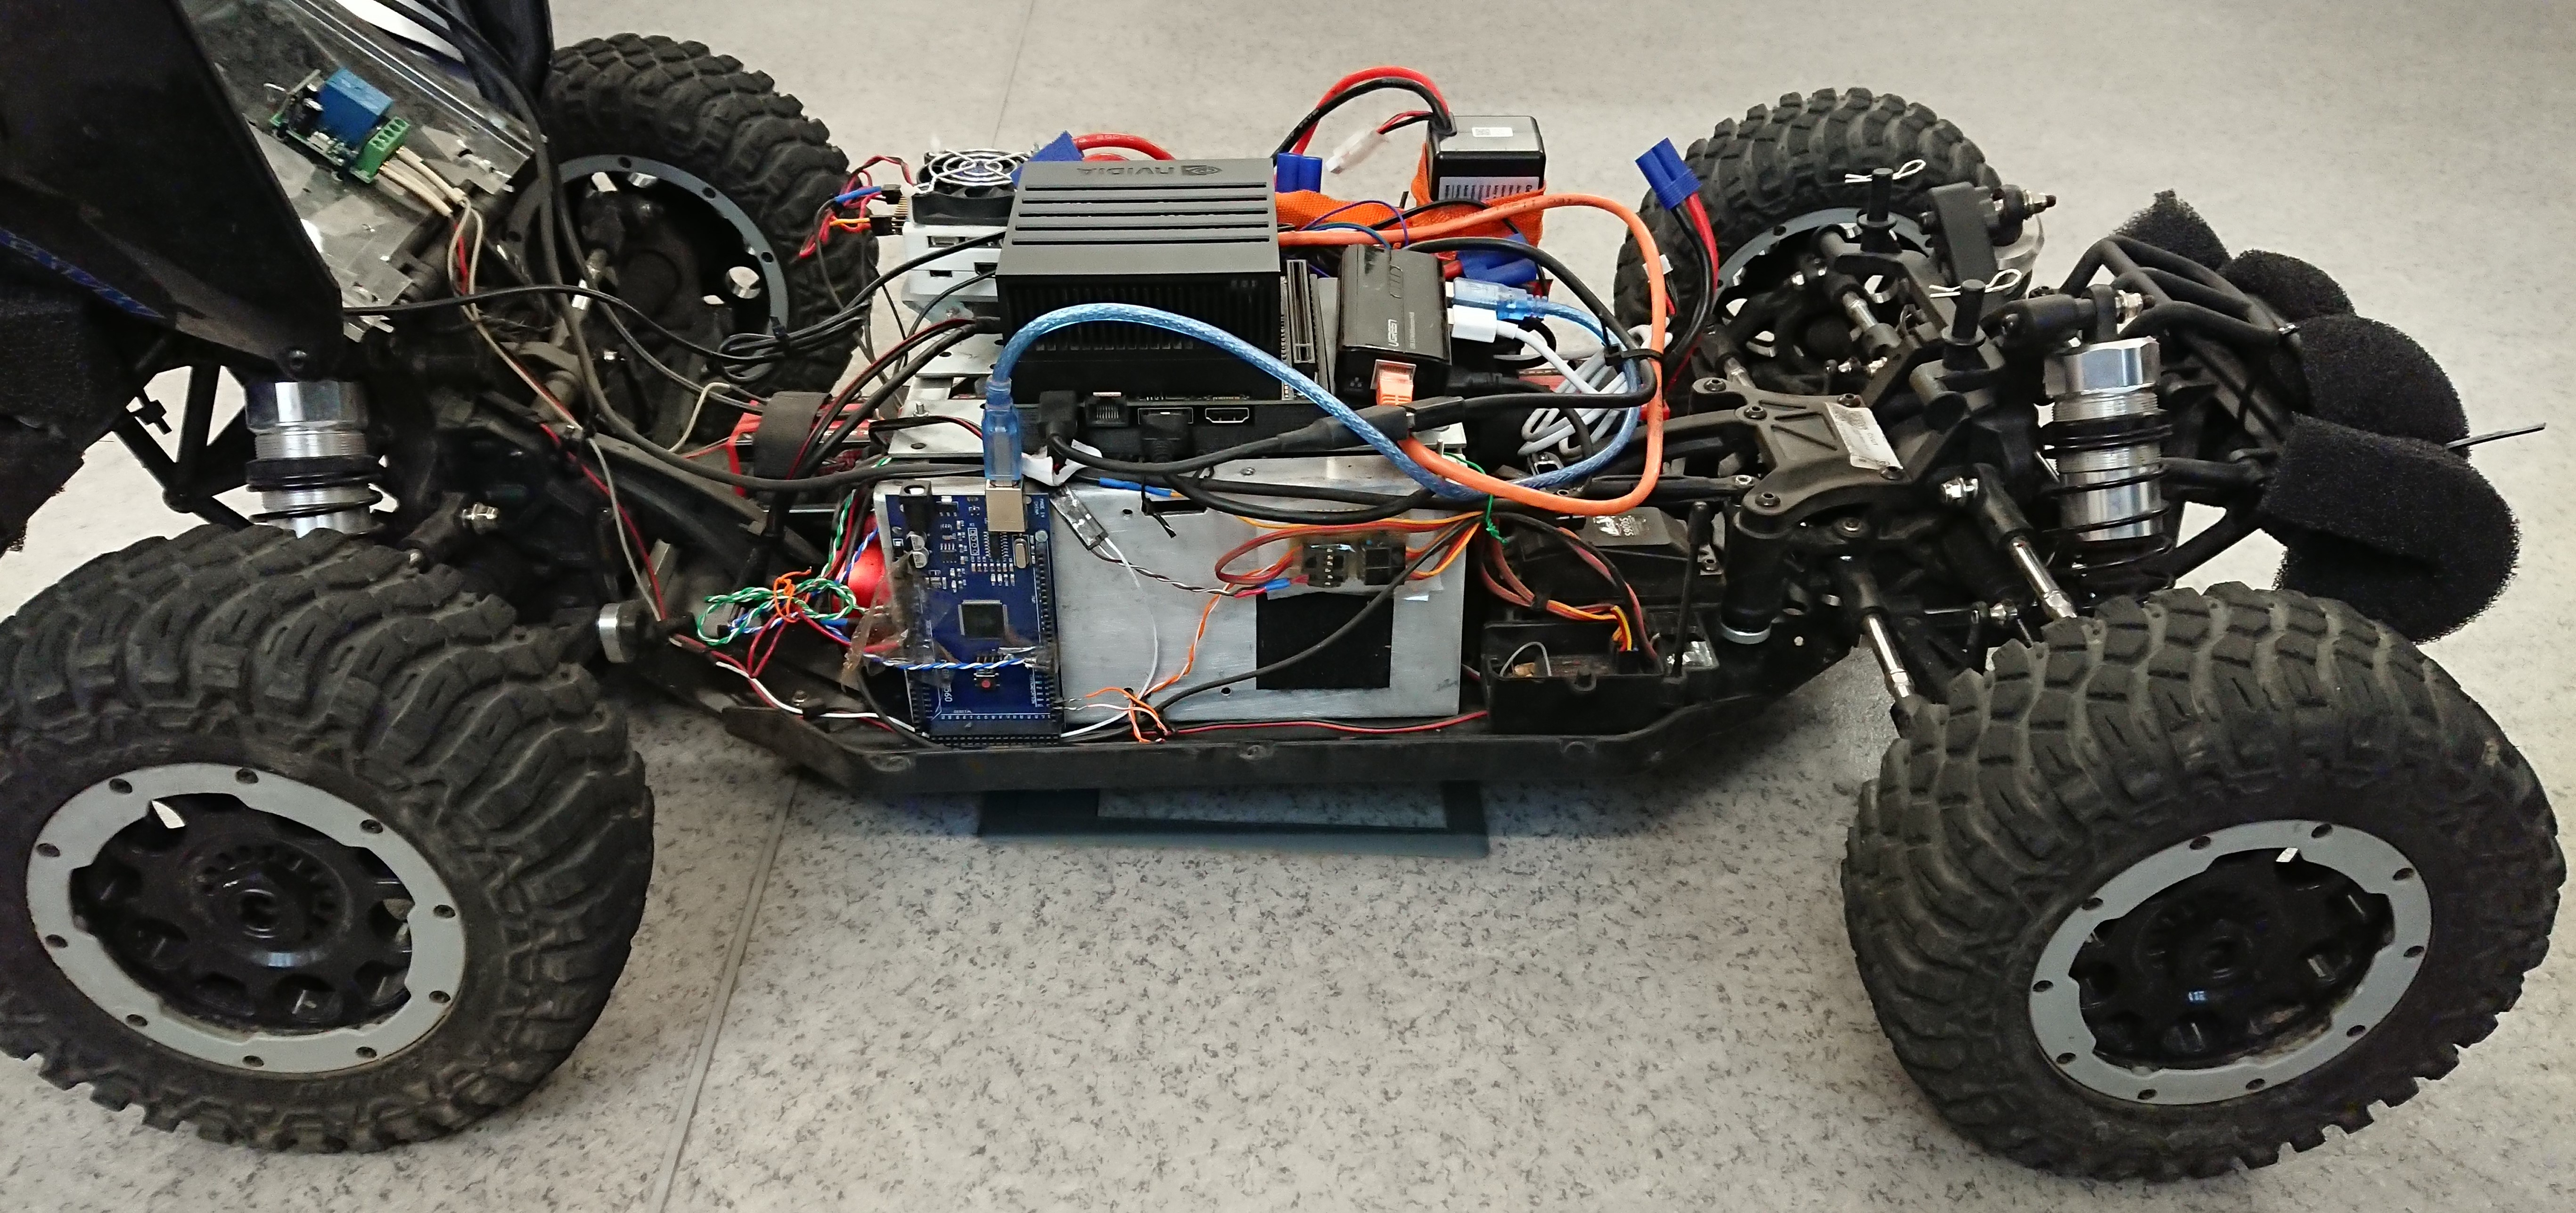
\includegraphics[width=.4\linewidth]{images/inside.jpg}
%\end{subfigure}
%\begin{subfigure}{0.5\textwidth}
%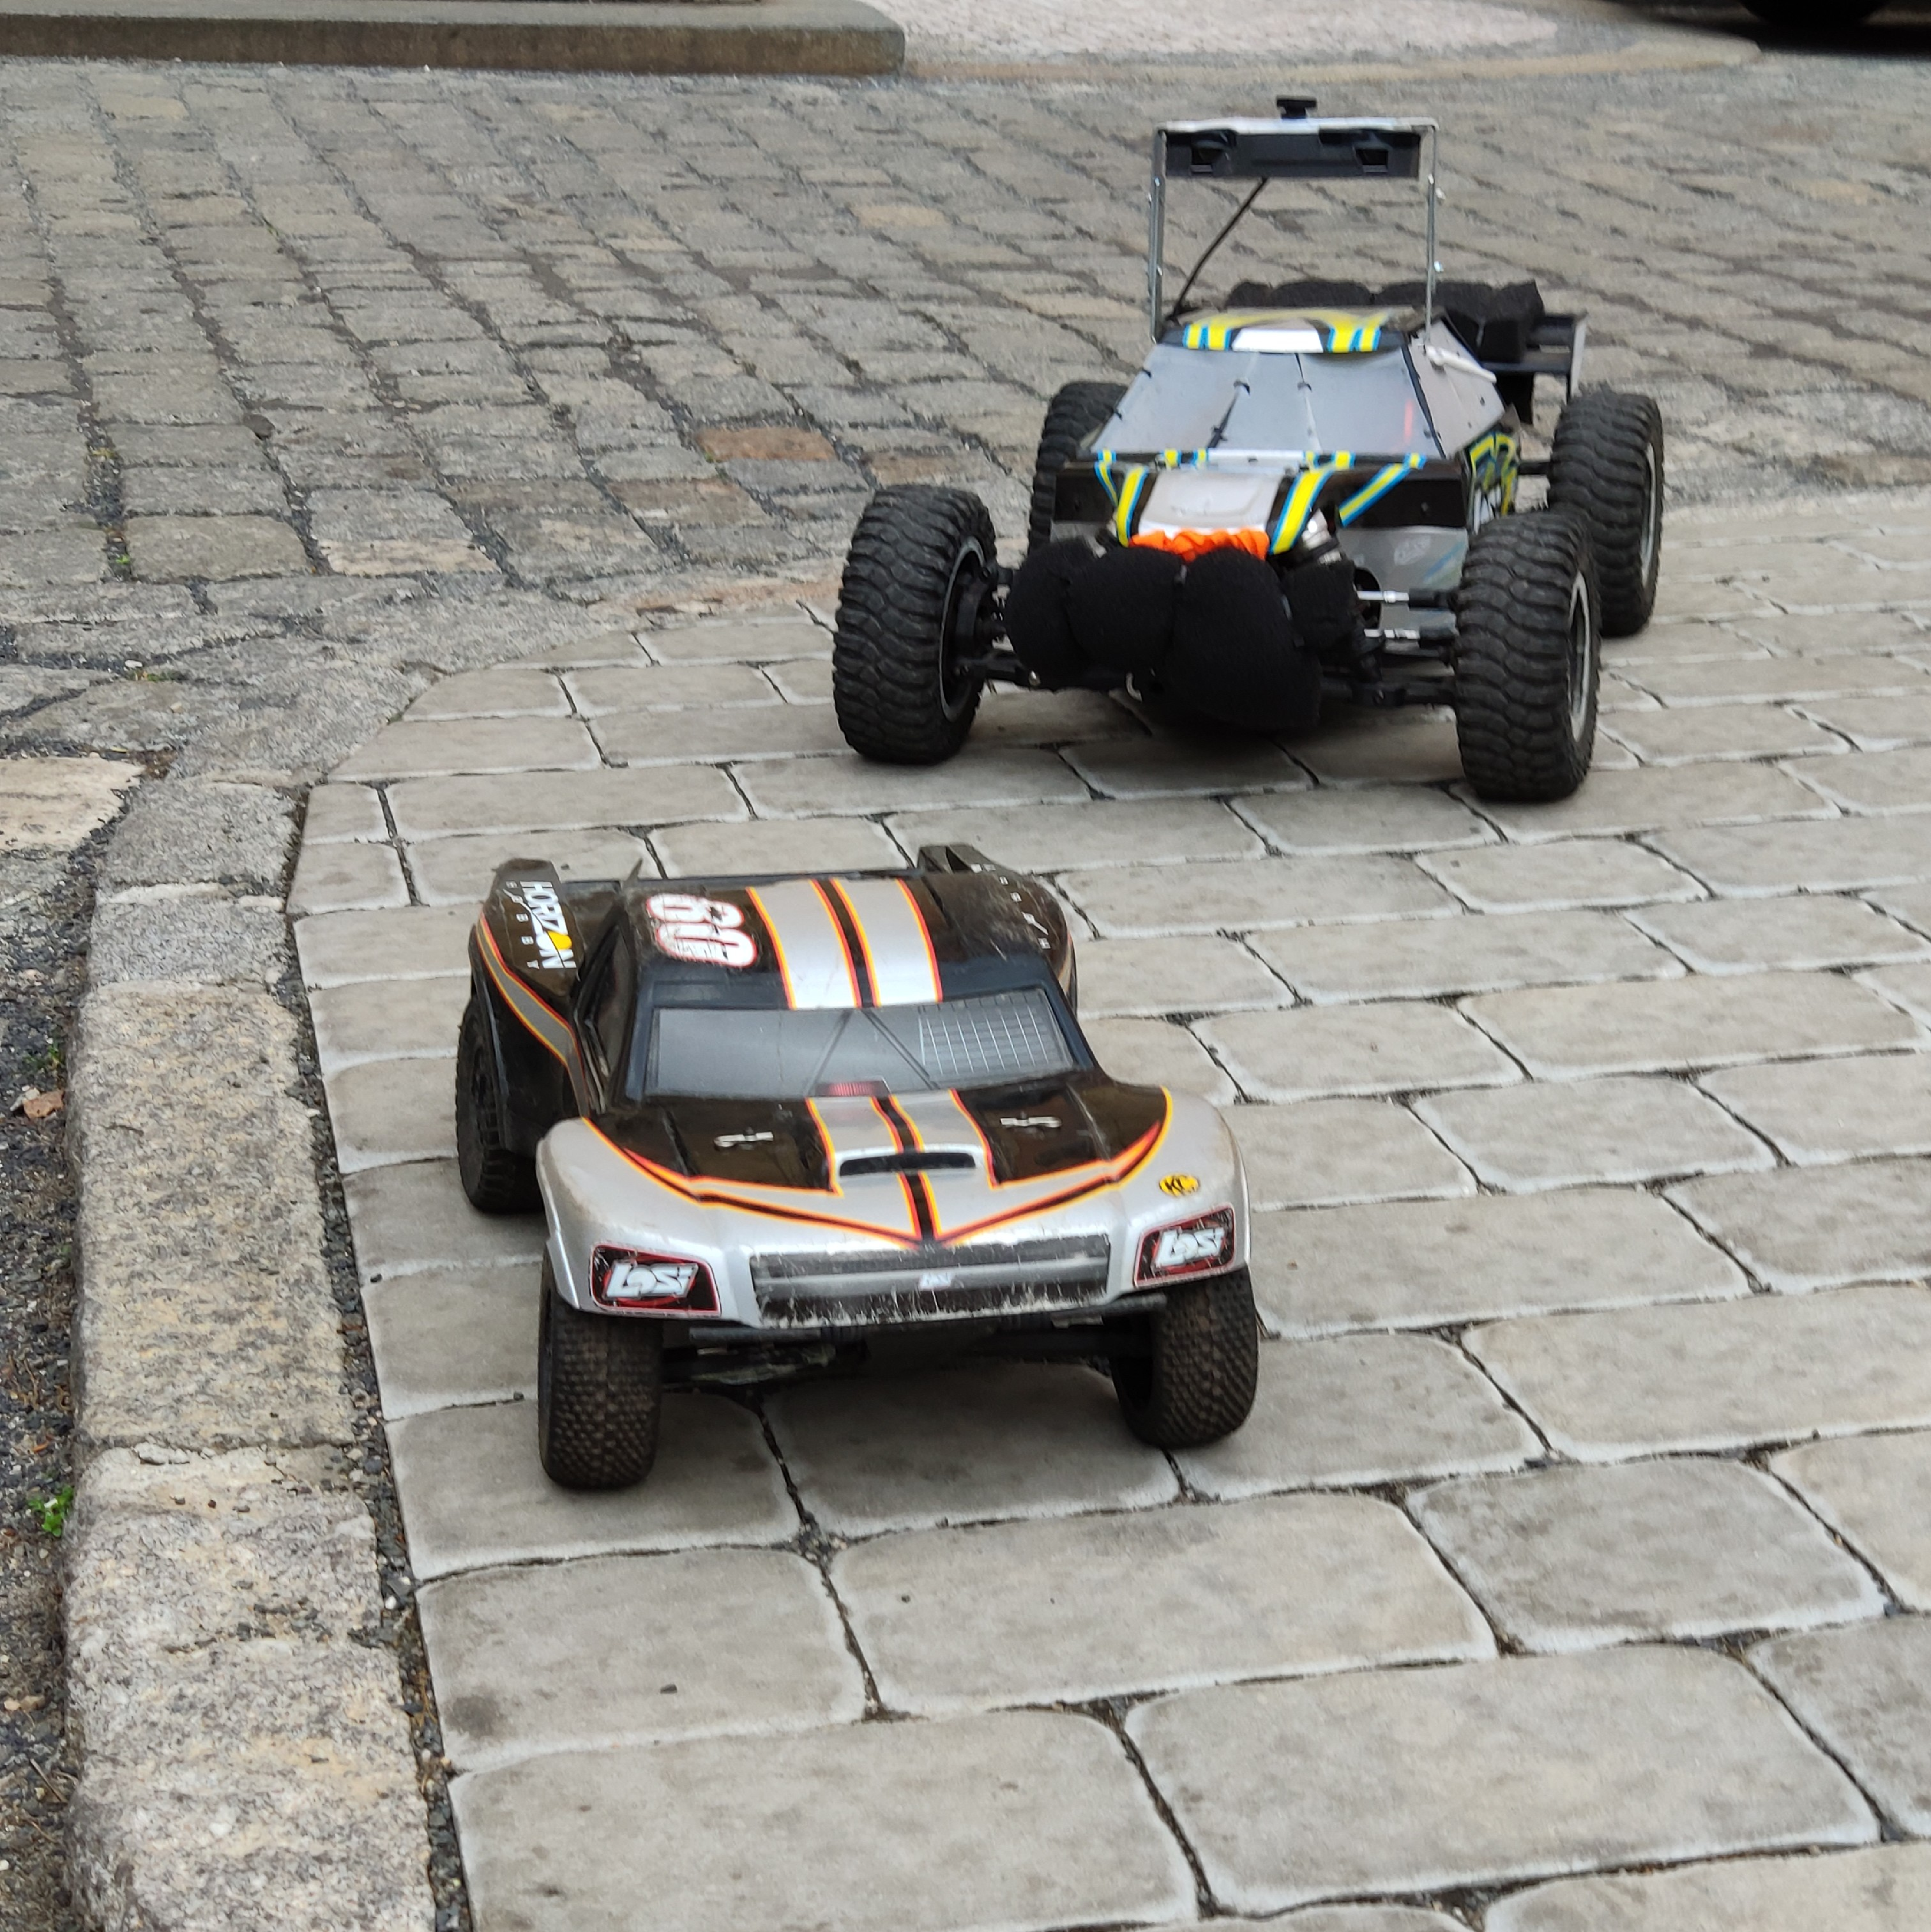
\includegraphics[width=.4\linewidth]{images/rc_cars.pdf}
%\end{subfigure}
%\caption{Both RC cars used for testing. The autonomous chasing car is in the back, while the manually driven car used as the pursued %car is in the front}
%\end{figure}


\subsubsection{Qualitative results}
We have performed live tests using a version of the system that did not have the dual-task neural network and therefore did not have the option to perform coarse semantic segmentation. The system was tested on an empty roundabout. During live tests, several safety measures were available. Multiple software conditions were implemented to stop the system. For example, in case the ZED camera stopped capturing images. We also limited the maximum speed of the autonomous vehicle. This was done by limiting the pulse width modulation (PWM) signals sent to the servo motor. On top of that, a remote emergency relay that can return manual control was available. We tested the system on multiple days during multiple weather conditions. The chasing trajectories driven on a road leading to the roundabout included a straight line and a U-turn. On the roundabout, the trajectories consisted of arc segments and full circles. \par


The autonomous system followed the other car smoothly without jerky movements. For the most part, it was able to successfully chase the other RC. It was maintaining the desired distance when chasing the other car on the roundabout as well as when the pursued car was driving in a straight line. If the chased car stopped, so did the autonomous system. The only limitation of the system comes from its current reactive nature, which in some instances affected the system's ability to perform U-turn on a narrow road. \par

The autonomous chase was documented and a highlight video is available online \cite{my_yt_video}.

\begin{figure}[]
    \centering
    \subfloat[Steer values in time]{{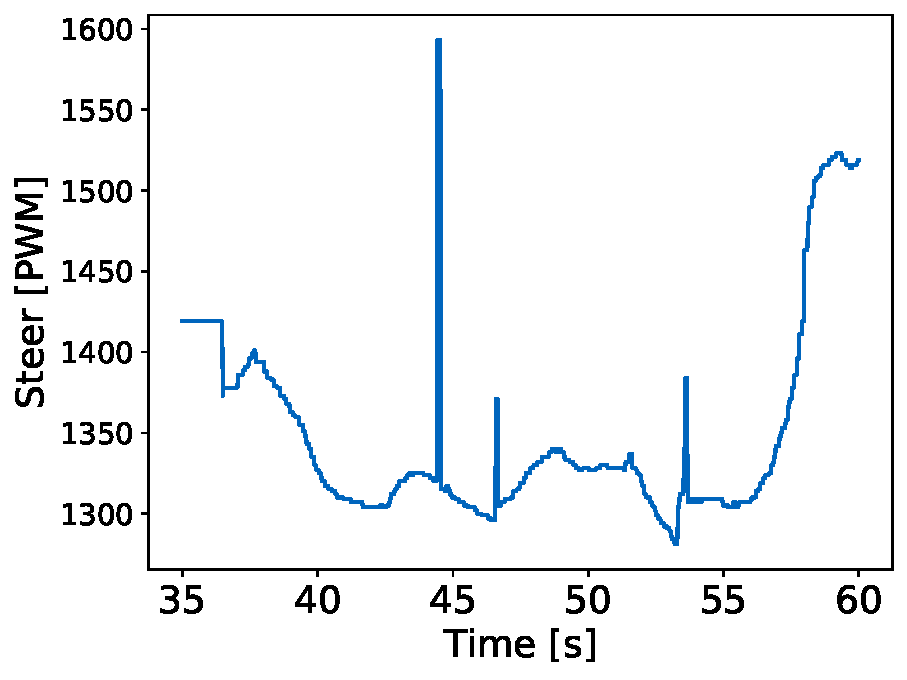
\includegraphics[width=0.45\textwidth]{images/steer_vid.pdf} }}%
    \quad
    \subfloat[Throttle in time]{{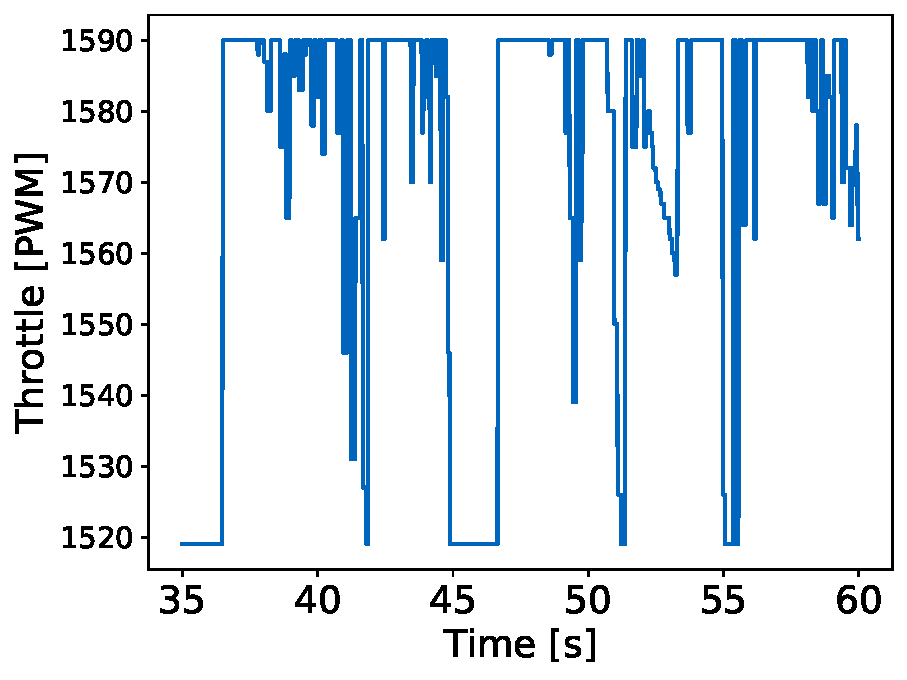
\includegraphics[width=0.45\textwidth]{images/throttle_vid.pdf} }}%
    \caption[Steer and throttle during autonomous RC car drive]{Steer and throttle PWM signals during the live test. The time in the graph corresponds to the time in the video of the live test \cite{my_yt_video}. The sudden spike in the graph \textbf{(a)} is caused by a false positive detection in a single frame}%
    \label{fig:prubeh}%
\end{figure}

\begin{figure}[]
    \centering
    \subfloat[Image taken at $t$ seconds]{{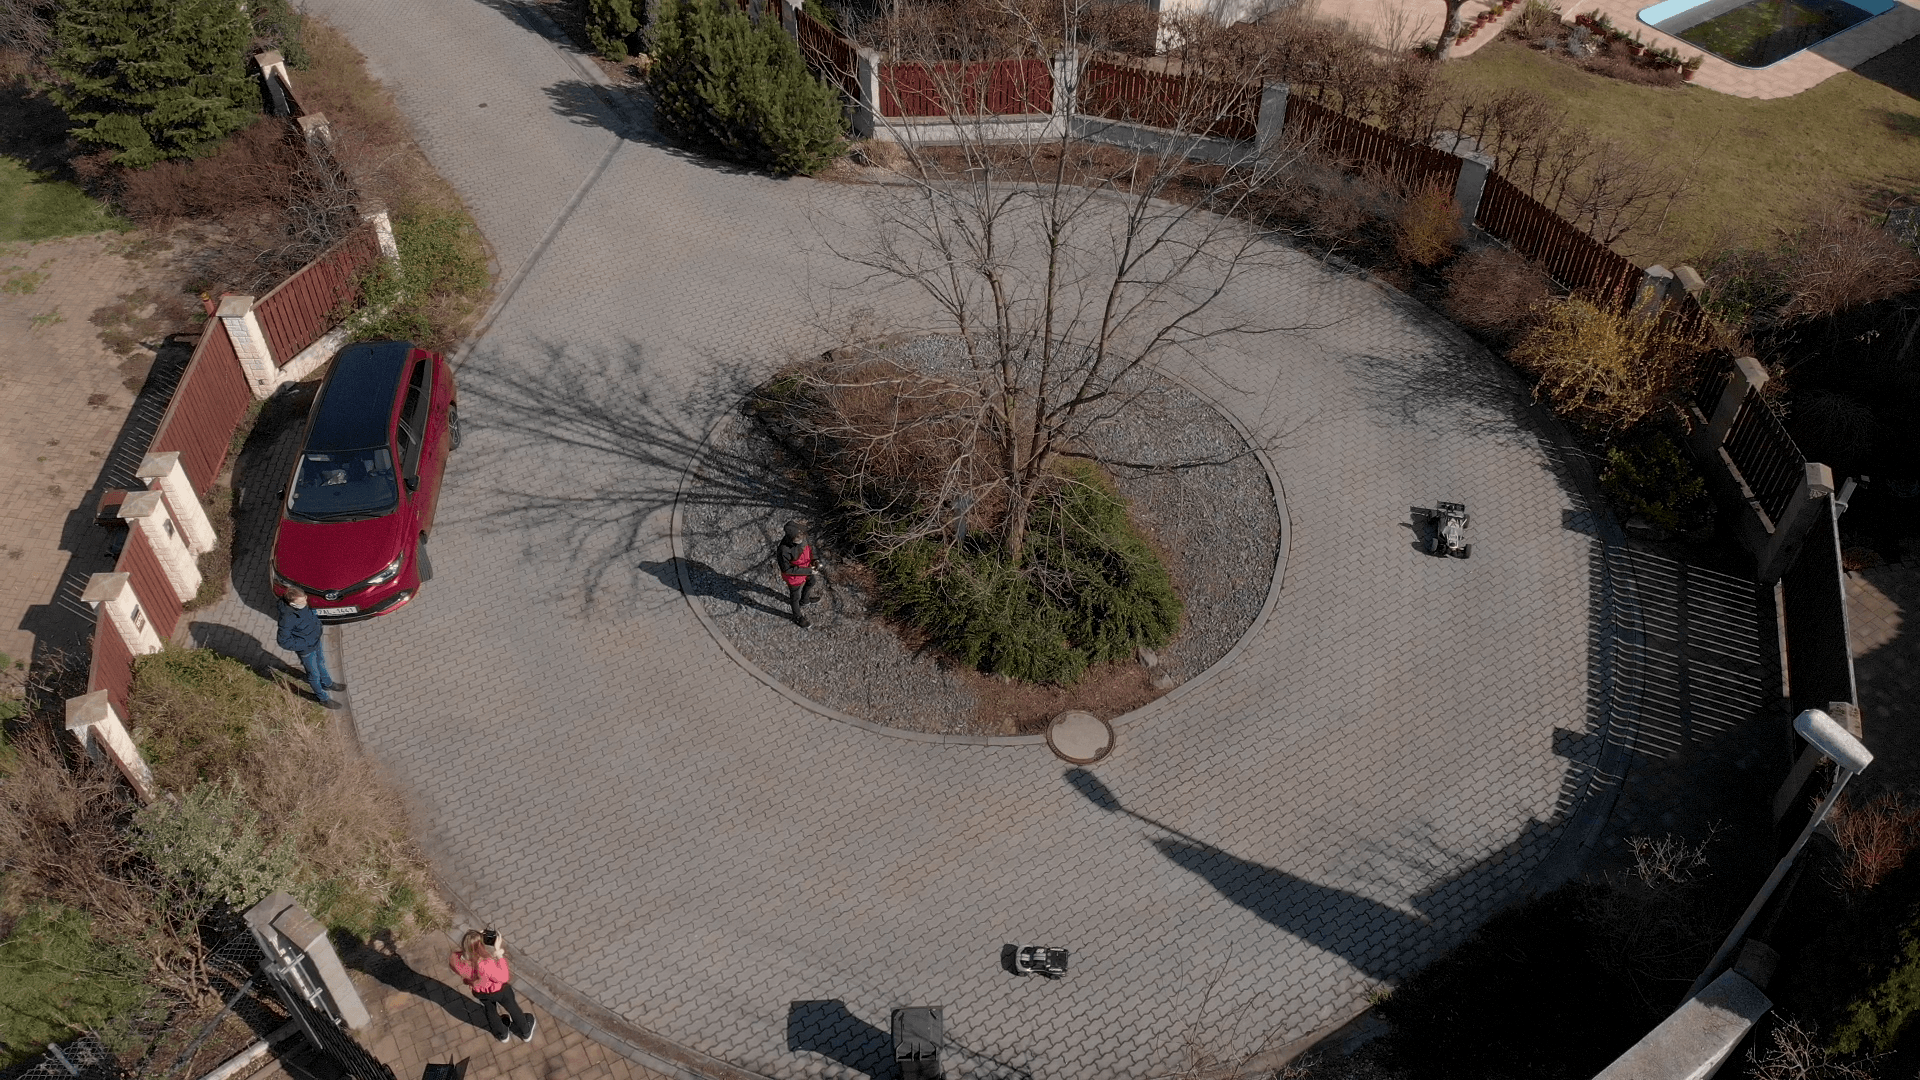
\includegraphics[width=1\textwidth]{images/drone_shot_2.4.2-optimized.png} }}%
    \quad
    \subfloat[Image taken at $t+1.9$ seconds]{{
    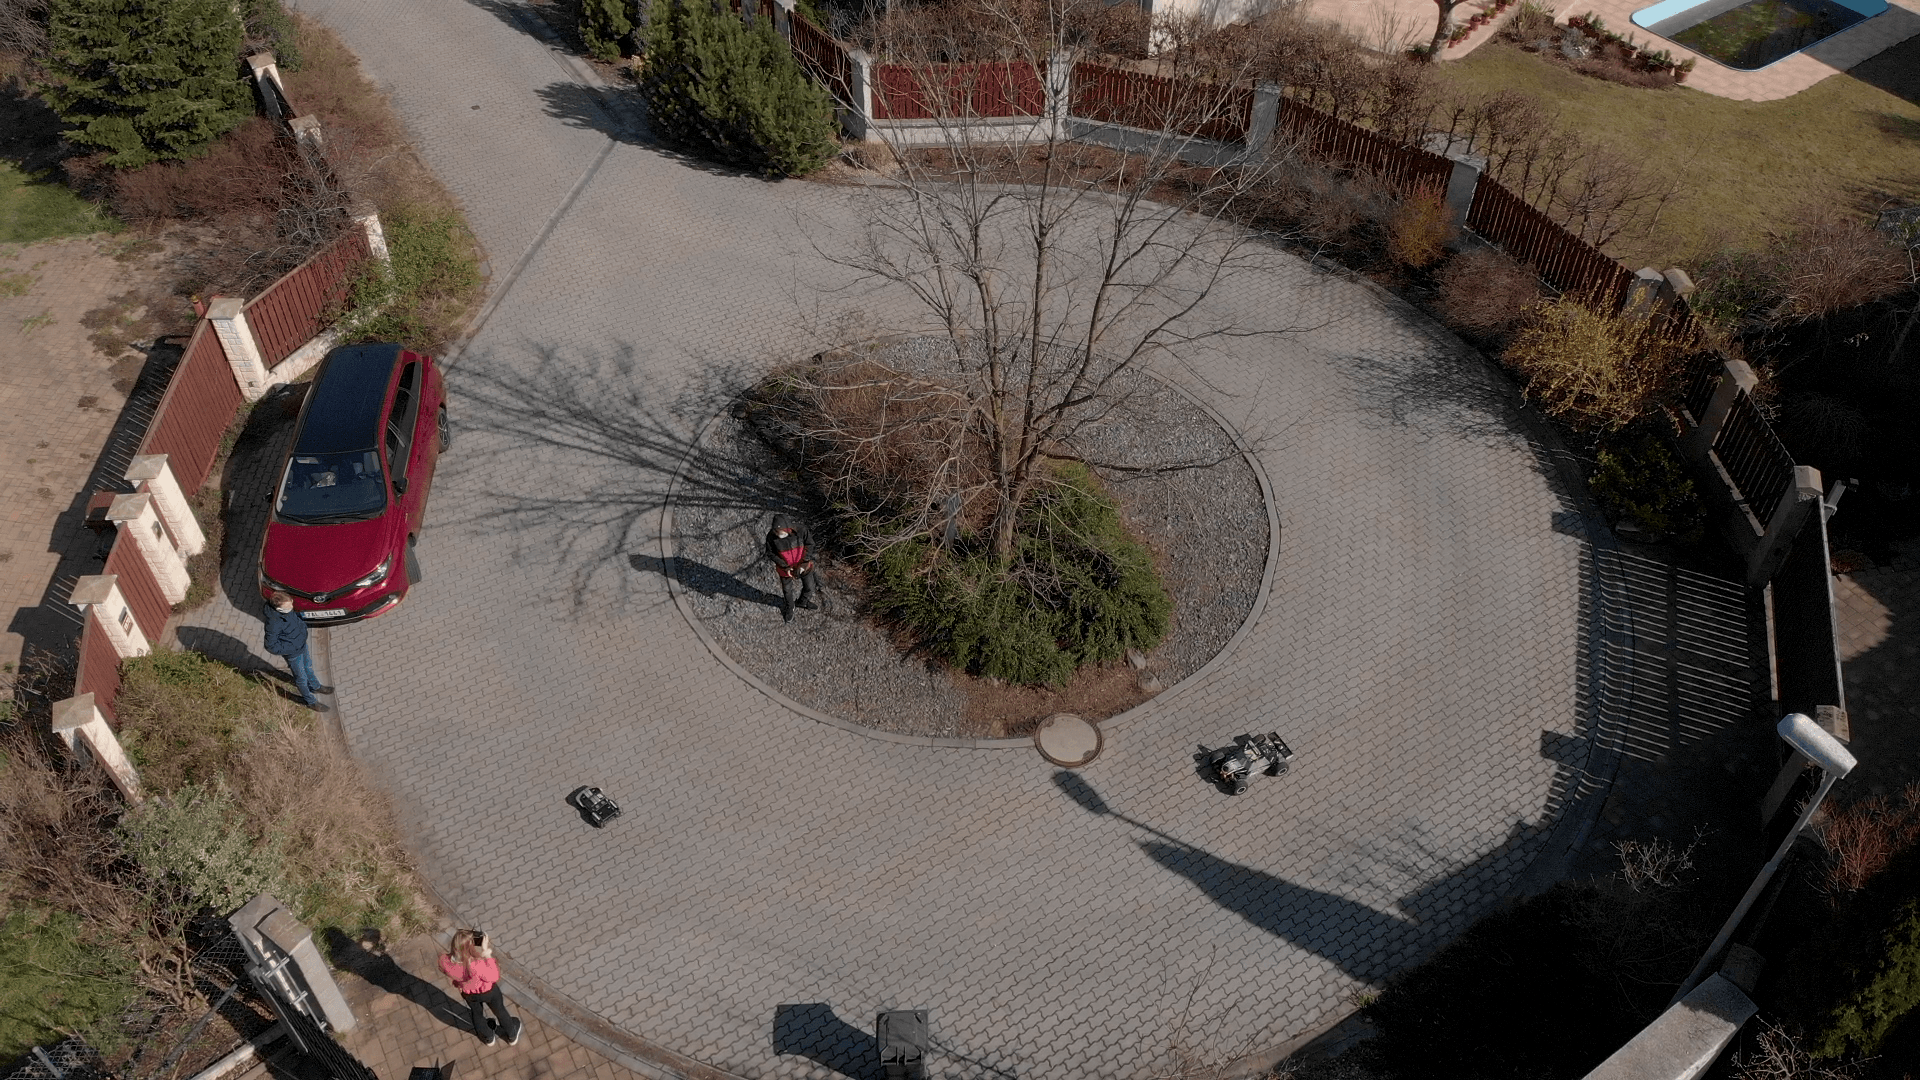
\includegraphics[width=1\textwidth]{images/drone_shot_2.4.3-optimized.png} }}%
    \caption[Drone photos of the live test.]{Drone photos of the live test. The RC car on the right is driven autonomously, while the RC car on the left is manually controlled with a transmitter. The person in the center of the image controls the chased car. The person closest to the red Toyota holds an emergency device that can stop the autonomous car and the third person controls the drone. Video of the autonomous car chase is available online \cite{my_yt_video}}\label{f:video}
\end{figure}






\chapter{Conclusion} \label{s:conclusion}
We have presented a novel dual-task convolutional neural network that concurrently detects objects and predicts coarse semantic segmentation. The network was trained using alternating optimization. We have developed a system, capable of autonomously chasing another vehicle, that uses the dual-task network. We have extensively evaluated different versions of the system in CARLA simulator. We have created a new challenging publicly available chasing dataset collected by manually driving the chased car. We have shown that the system benefits from using the coarse semantic segmentation. Especially if the detector has low detection recall.\par
We have collected and annotated three new publicly available datasets \cite{my_github}. In addition to the CARLA driving set, we have collected an object detection dataset consisting of 460 images of a pursued RC car as well as a semantic segmentation dataset consisting of 460 images segmented into drivable and non-drivable parts. \par
Finally, we have implemented the system on a subscale vehicle platform built on a high-speed RC car. We have demonstrated and documented \cite{my_yt_video} the system's ability to chase another car.\par
Currently, the system shows robust chasing capabilities despite using only information from a single RGB camera. One of the system limitations is its reactive nature. We believe that the system could improve by using a more sophisticated trajectory planning algorithm that would include predictive modeling of the chased car. In the future, we would also like to evaluate the system more extensively with RC cars.

\bibliography{citations}
\bibliographystyle{IEEEtran}

\end{document}

